%======================================================================
% CAPITULO 5: VISOR DE DOCUMENTOS SEGURO
%======================================================================

\chapter{Visor de Documentos Seguro}
\label{ch:visor}

Una de las caracteristicas exclusivas de \sdc{} es el \textbf{Visor Seguro}, que permite visualizar documentos confidenciales sin dejar rastro fisico en el disco duro.

\section{Visor Seguro de SDC}
\label{sec:visor-seguro}

El visor implementa un modelo de seguridad unico: los documentos se desencriptan directamente en la memoria RAM y nunca se escriben en el almacenamiento persistente.

\begin{figure}[H]
\centering
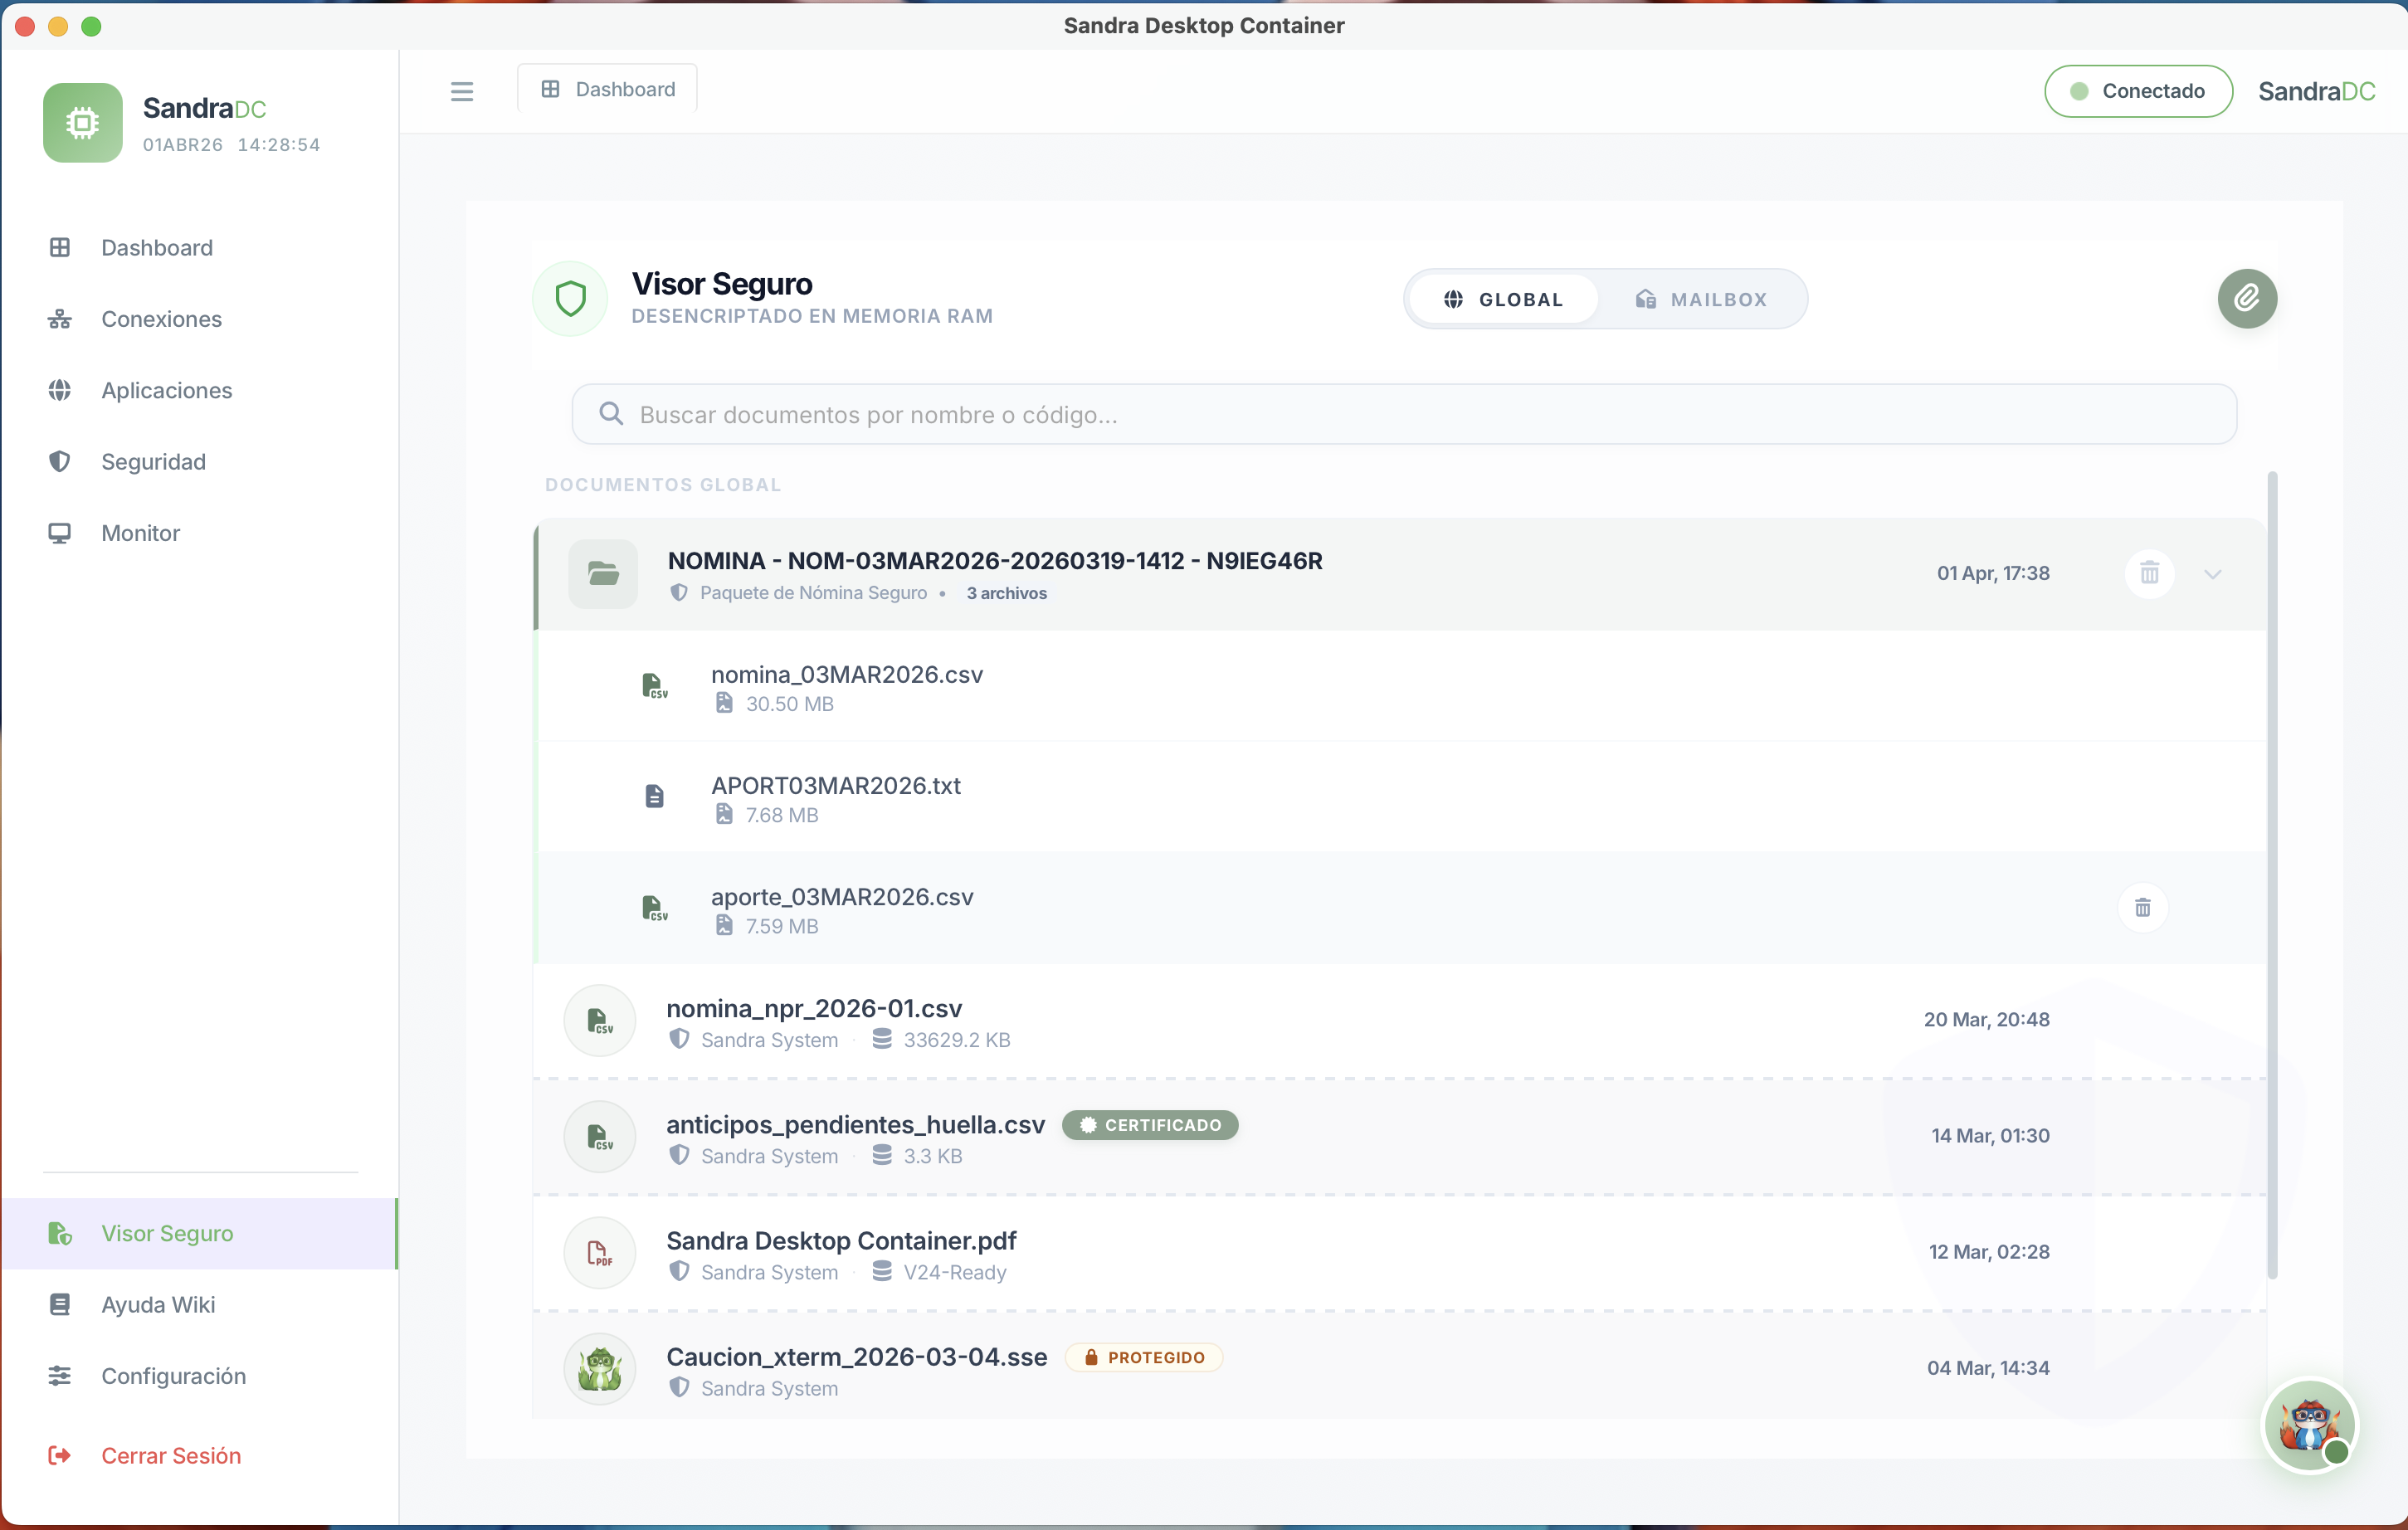
\includegraphics[width=0.95\textwidth]{anexos/11 visor.png}
\caption{Visor seguro de documentos}
\label{fig:visor}
\end{figure}

\subsection{Principio de Operacion}

\begin{enumerate}[leftmargin=*]
    \item El documento encriptado se transfiere desde el servidor origen
    \item Se descifra en tiempo real usando la clave privada del Client ID
    \item El contenido plano se mantiene unicamente en buffers de memoria RAM
    \item Se renderiza en el visor sin crear archivos temporales
    \item Al cerrar, los buffers se sobrescriben con ceros (zero-fill)
\end{enumerate}

\begin{quote}
\textbf{Proteccion Forense}\\
Al cerrar el visor, no queda rastro fisico del archivo en el disco duro. Esto evita la fuga de datos mediante tecnicas de analisis forense digital.
\end{quote}

\section{Formatos Soportados}
\label{sec:formatos}

El visor soporta multiples formatos de documento:

\begin{table}[H]
\centering
\begin{tabular}{p{4cm}p{3cm}p{6cm}}
\toprule
\textbf{Formato} & \textbf{Extension} & \textbf{Caracteristicas} \\
\midrule
PDF & .pdf & Visualizacion nativa con anotaciones \\
\midrule
Imagenes & .png, .jpg, .gif & Zoom, rotacion, filtros \\
\midrule
Documentos Office & .docx, .xlsx & Renderizado simplificado \\
\midrule
Texto Plano & .txt, .md, .json & Sintaxis resaltada \\
\midrule
Codigo Fuente & .rs, .ts, .js & Coloreado por lenguaje \\
\bottomrule
\end{tabular}
\caption{Formatos de documento soportados por el visor}
\label{tab:formatos}
\end{table}

\section{Lista de Documentos}
\label{sec:lista-documentos}

El panel de lista muestra todos los documentos disponibles.

\begin{figure}[H]
\centering
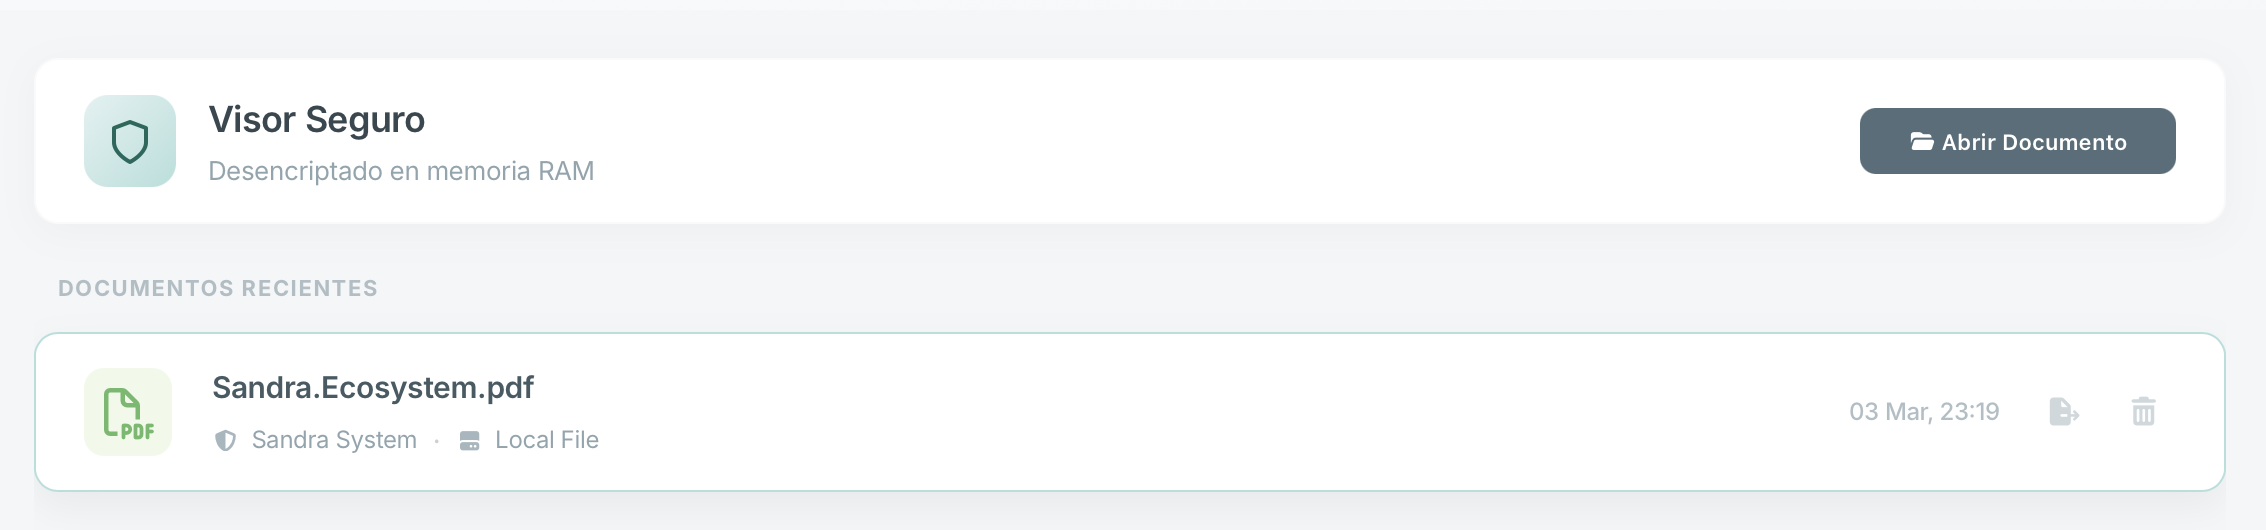
\includegraphics[width=0.95\textwidth]{anexos/13 visor list.png}
\caption{Lista de documentos en el visor}
\label{fig:visor-lista}
\end{figure}

\subsection{Informacion Visualizada}

Para cada documento se muestra:

\begin{itemize}[leftmargin=*]
    \item Nombre del archivo
    \item Tamanio en formato legible
    \item Fecha de ultima modificacion
    \item Estado de encriptacion (Verde: Encriptado)
    \item Propietario o autor
    \item Etiquetas de clasificacion
\end{itemize}

\section{Flujo de Encriptacion GPG}
\label{sec:gpg}

SDC implementa un sistema de encriptacion hibrido basado en \textbf{GPG} (GNU Privacy Guard), el estandar de facto para comunicaciones seguras.

\begin{figure}[H]
\centering
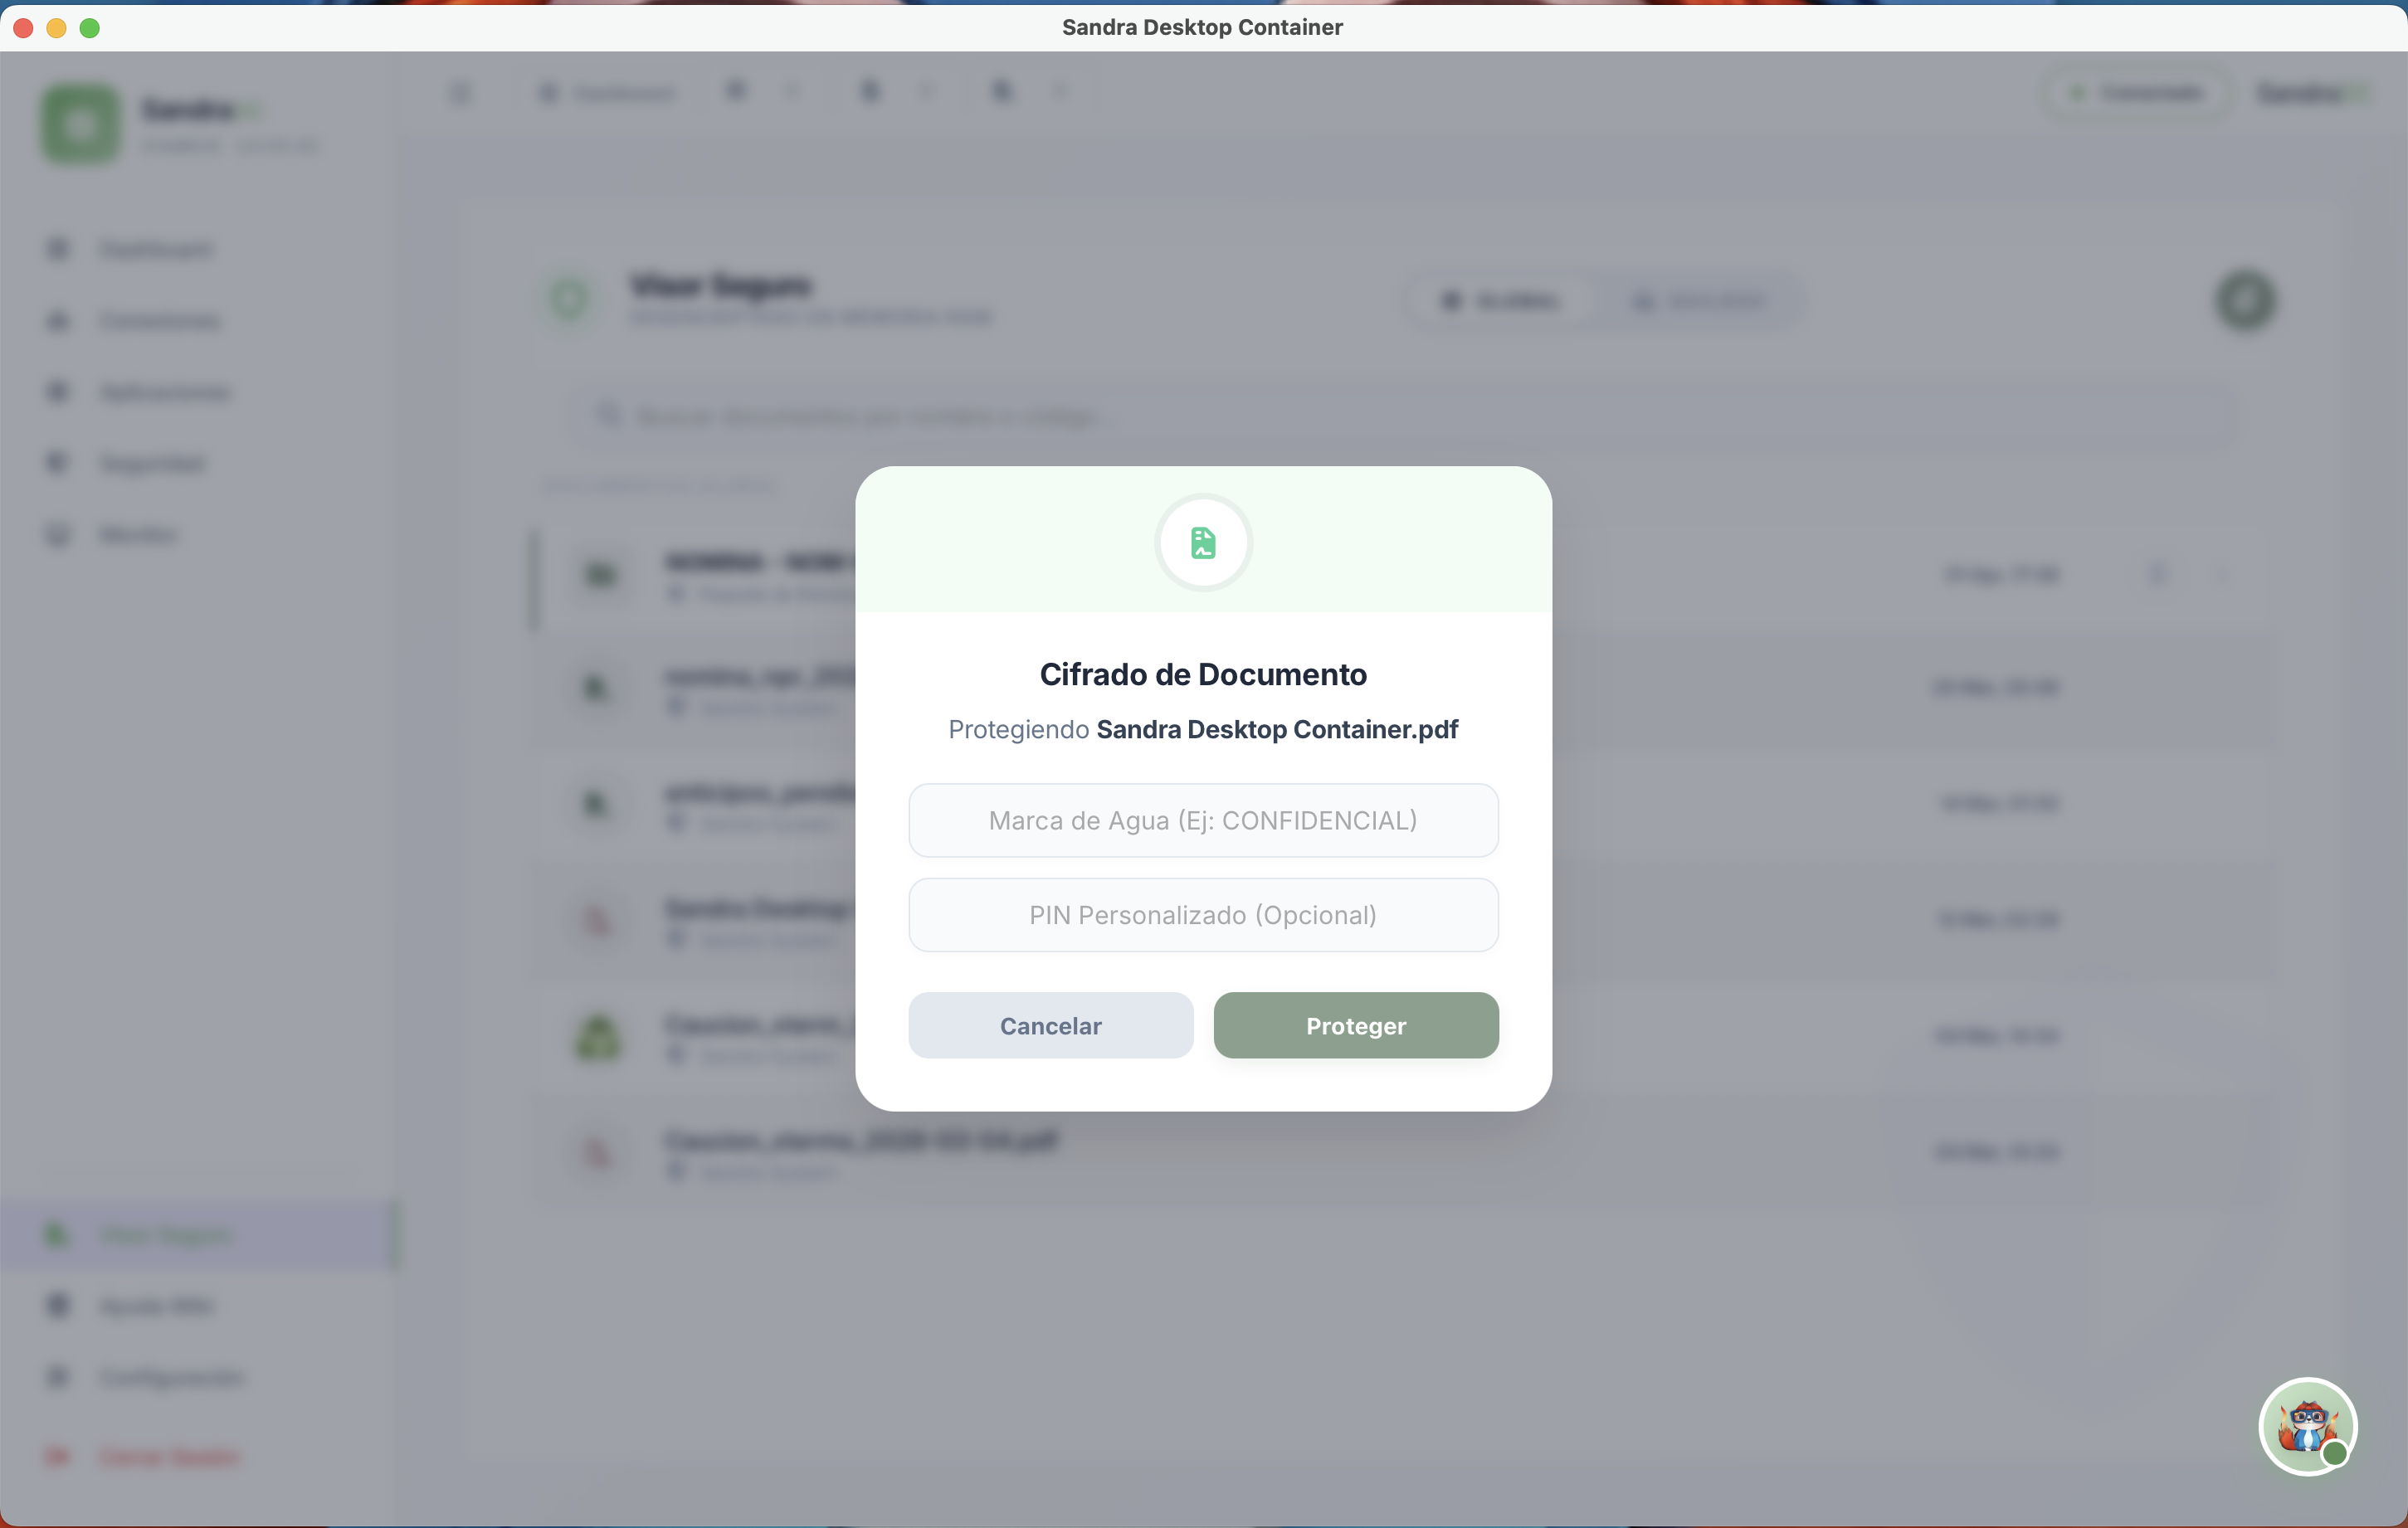
\includegraphics[width=0.95\textwidth]{anexos/11 visor encriptar.png}
\caption{Proceso de encriptacion de documento}
\label{fig:visor-encriptar}
\end{figure}

\subsection{Historia y Contexto de GPG}

GPG nacio en 1997 como implementacion libre del estandar \textbf{OpenPGP} (RFC 4880). Fue creado por Werner Koch como alternativa libre al software PGP (Pretty Good Privacy) de Phil Zimmermann, que en aquel entonces estaba sujeto a restricciones de exportacion de criptografia desde Estados Unidos.

\begin{quote}
\textbf{Relevancia Historica}\\
GPG se ha convertido en el estandar de facto para:
\begin{itemize}
    \item Firma de codigo fuente en proyectos de software libre
    \item Comunicaciones seguras en activismo y periodismo
    \item Proteccion de datos en entornos empresariales
    \item Verificacion de integridad en distribuciones de software
\end{itemize}
\end{quote}

\subsection{Fundamentos Criptograficos}

GPG utiliza un esquema hibrido que combina lo mejor de dos mundos:

\begin{enumerate}
    \item \textbf{Cifrado Simetrico (AES-256-GCM)}: Rapido y eficiente para grandes volumenes de datos
    \item \textbf{Cifrado Asimetrico (RSA-4096)}: Seguro para intercambio de claves entre partes
\end{enumerate}

\begin{quote}
\textbf{Ventajas del Esquema Hibrido}\\
\begin{itemize}
    \item \textbf{Velocidad}: El cifrado simetrico es miles de veces mas rapido que el asimetrico
    \item \textbf{Seguridad}: Las claves asimetricas permiten compartir sin exponer el secreto
    \item \textbf{Escalabilidad}: Documentos de cualquier tamano pueden protegerse eficientemente
    \item \textbf{Autenticacion}: Las firmas digitales garantizan la identidad del emisor
\end{itemize}
\end{quote}

\subsection{Proceso de Encriptacion en SDC}

\begin{figure}[H]
\centering
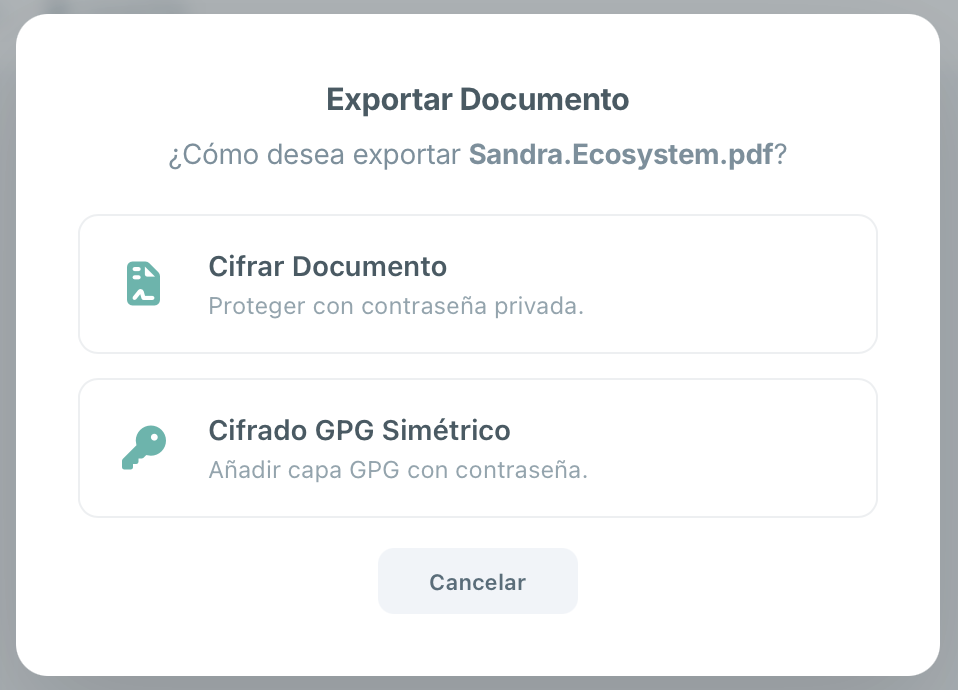
\includegraphics[width=0.95\textwidth]{anexos/14 visor encriptado.png}
\caption{Documento en estado encriptado}
\label{fig:visor-encriptado}
\end{figure}

El proceso de encriptacion en SDC sigue estos pasos:

\begin{enumerate}[leftmargin=*]
    \item \textbf{Generacion de Clave de Sesion}: Se crea una clave AES-256 aleatoria (32 bytes) unica para este documento
    \item \textbf{Cifrado del Contenido}: El documento se cifra usando AES-256-GCM con la clave de sesion
    \item \textbf{Proteccion de Clave}: La clave de sesion se cifra con la clave publica RSA-4096 del destinatario
    \item \textbf{Empaquetado}: Se combina el documento cifrado, la clave cifrada y los metadatos
    \item \textbf{Firma Digital}: El paquete se firma con la clave privada del emisor para garantizar autenticidad
\end{enumerate}

\subsection{Relevancia para SandraDC}

La implementacion GPG en SDC proporciona:

\begin{itemize}[leftmargin=*]
    \item \textbf{Confidencialidad}: Solo el destinatario autorizado puede descifrar el contenido
    \item \textbf{Integridad}: Cualquier modificacion del archivo invalida la firma digital
    \item \textbf{Autenticidad}: La firma garantiza que el documento proviene del emisor declarado
    \item \textbf{No repudio}: El emisor no puede negar haber enviado el documento firmado
    \item \textbf{Interoperabilidad}: Los documentos pueden intercambiarse con otros sistemas GPG/PGP
\end{itemize}

\section{Exportacion y Compartir}
\label{sec:exportar}

SDC permite exportar documentos de forma segura para compartirlos con otros usuarios o sistemas.

\begin{figure}[H]
\centering
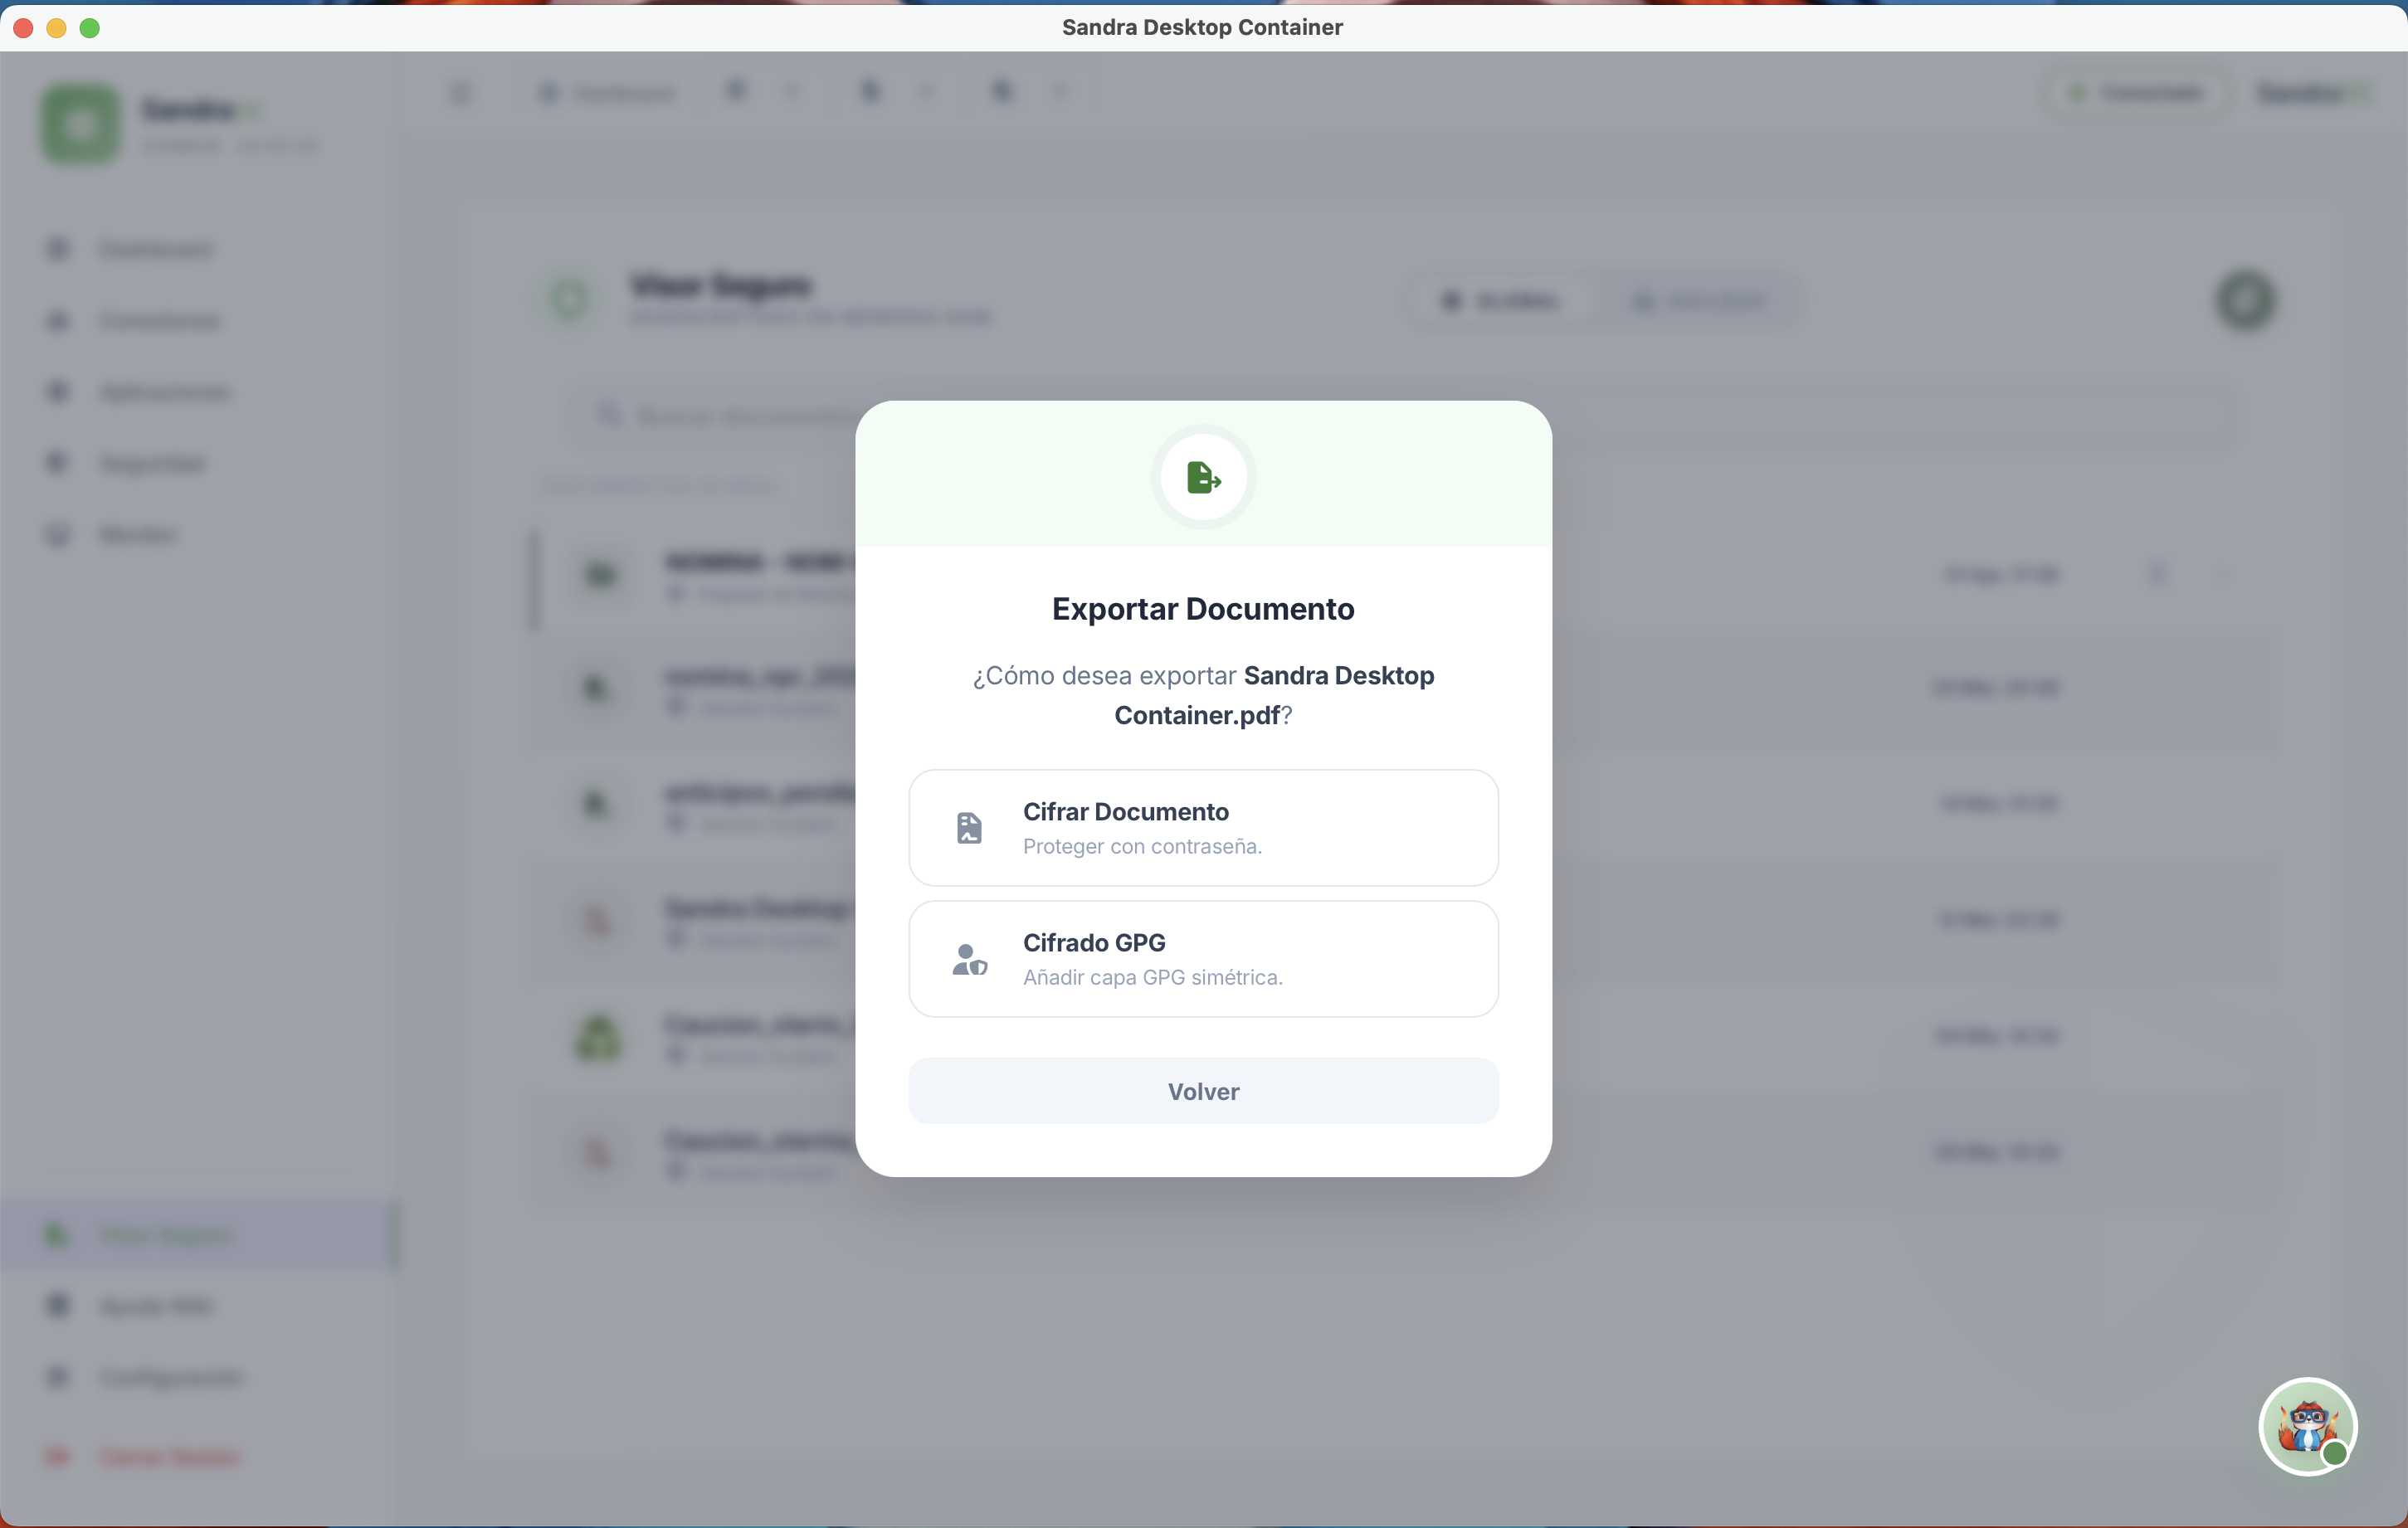
\includegraphics[width=0.95\textwidth]{anexos/11 visor exportar.png}
\caption{Opciones de exportacion segura}
\label{fig:visor-exportar}
\end{figure}

\subsection{Opciones de Exportacion}

\begin{table}[H]
\centering
\begin{tabular}{p{4cm}p{4cm}p{6cm}}
\toprule
\textbf{Metodo} & \textbf{Formato} & \textbf{Uso Recomendado} \\
\midrule
Exportar Encriptado & .gpg / .pgp & Para transferencia segura \\
\midrule
Exportar Firmado & .sig adjunto & Para verificacion de integridad \\
\midrule
Exportar ZIP & .zip encriptado & Para multiples archivos \\
\midrule
Compartir Link & URL temporal & Para acceso controlado \\
\bottomrule
\end{tabular}
\caption{Metodos de exportacion disponibles}
\label{tab:exportar}
\end{table}

\begin{quote}
\textbf{Enlaces Temporales}\\
Al compartir mediante link, SDC genera una URL unica con:
\begin{itemize}
    \item Expiracion configurable (1 hora a 30 dias)
    \item Limite de descargas
    \item Registro de auditoria de accesos
    \item Revocacion instantanea si es necesario
\end{itemize}
\end{quote}

\section{Previsualizacion de Documentos}
\label{sec:preview}

El visor ofrece un sistema de previsualizacion que permite verificar el contenido antes de desbloquearlo completamente.

\subsection{Documento Protegido}

\begin{figure}[H]
\centering
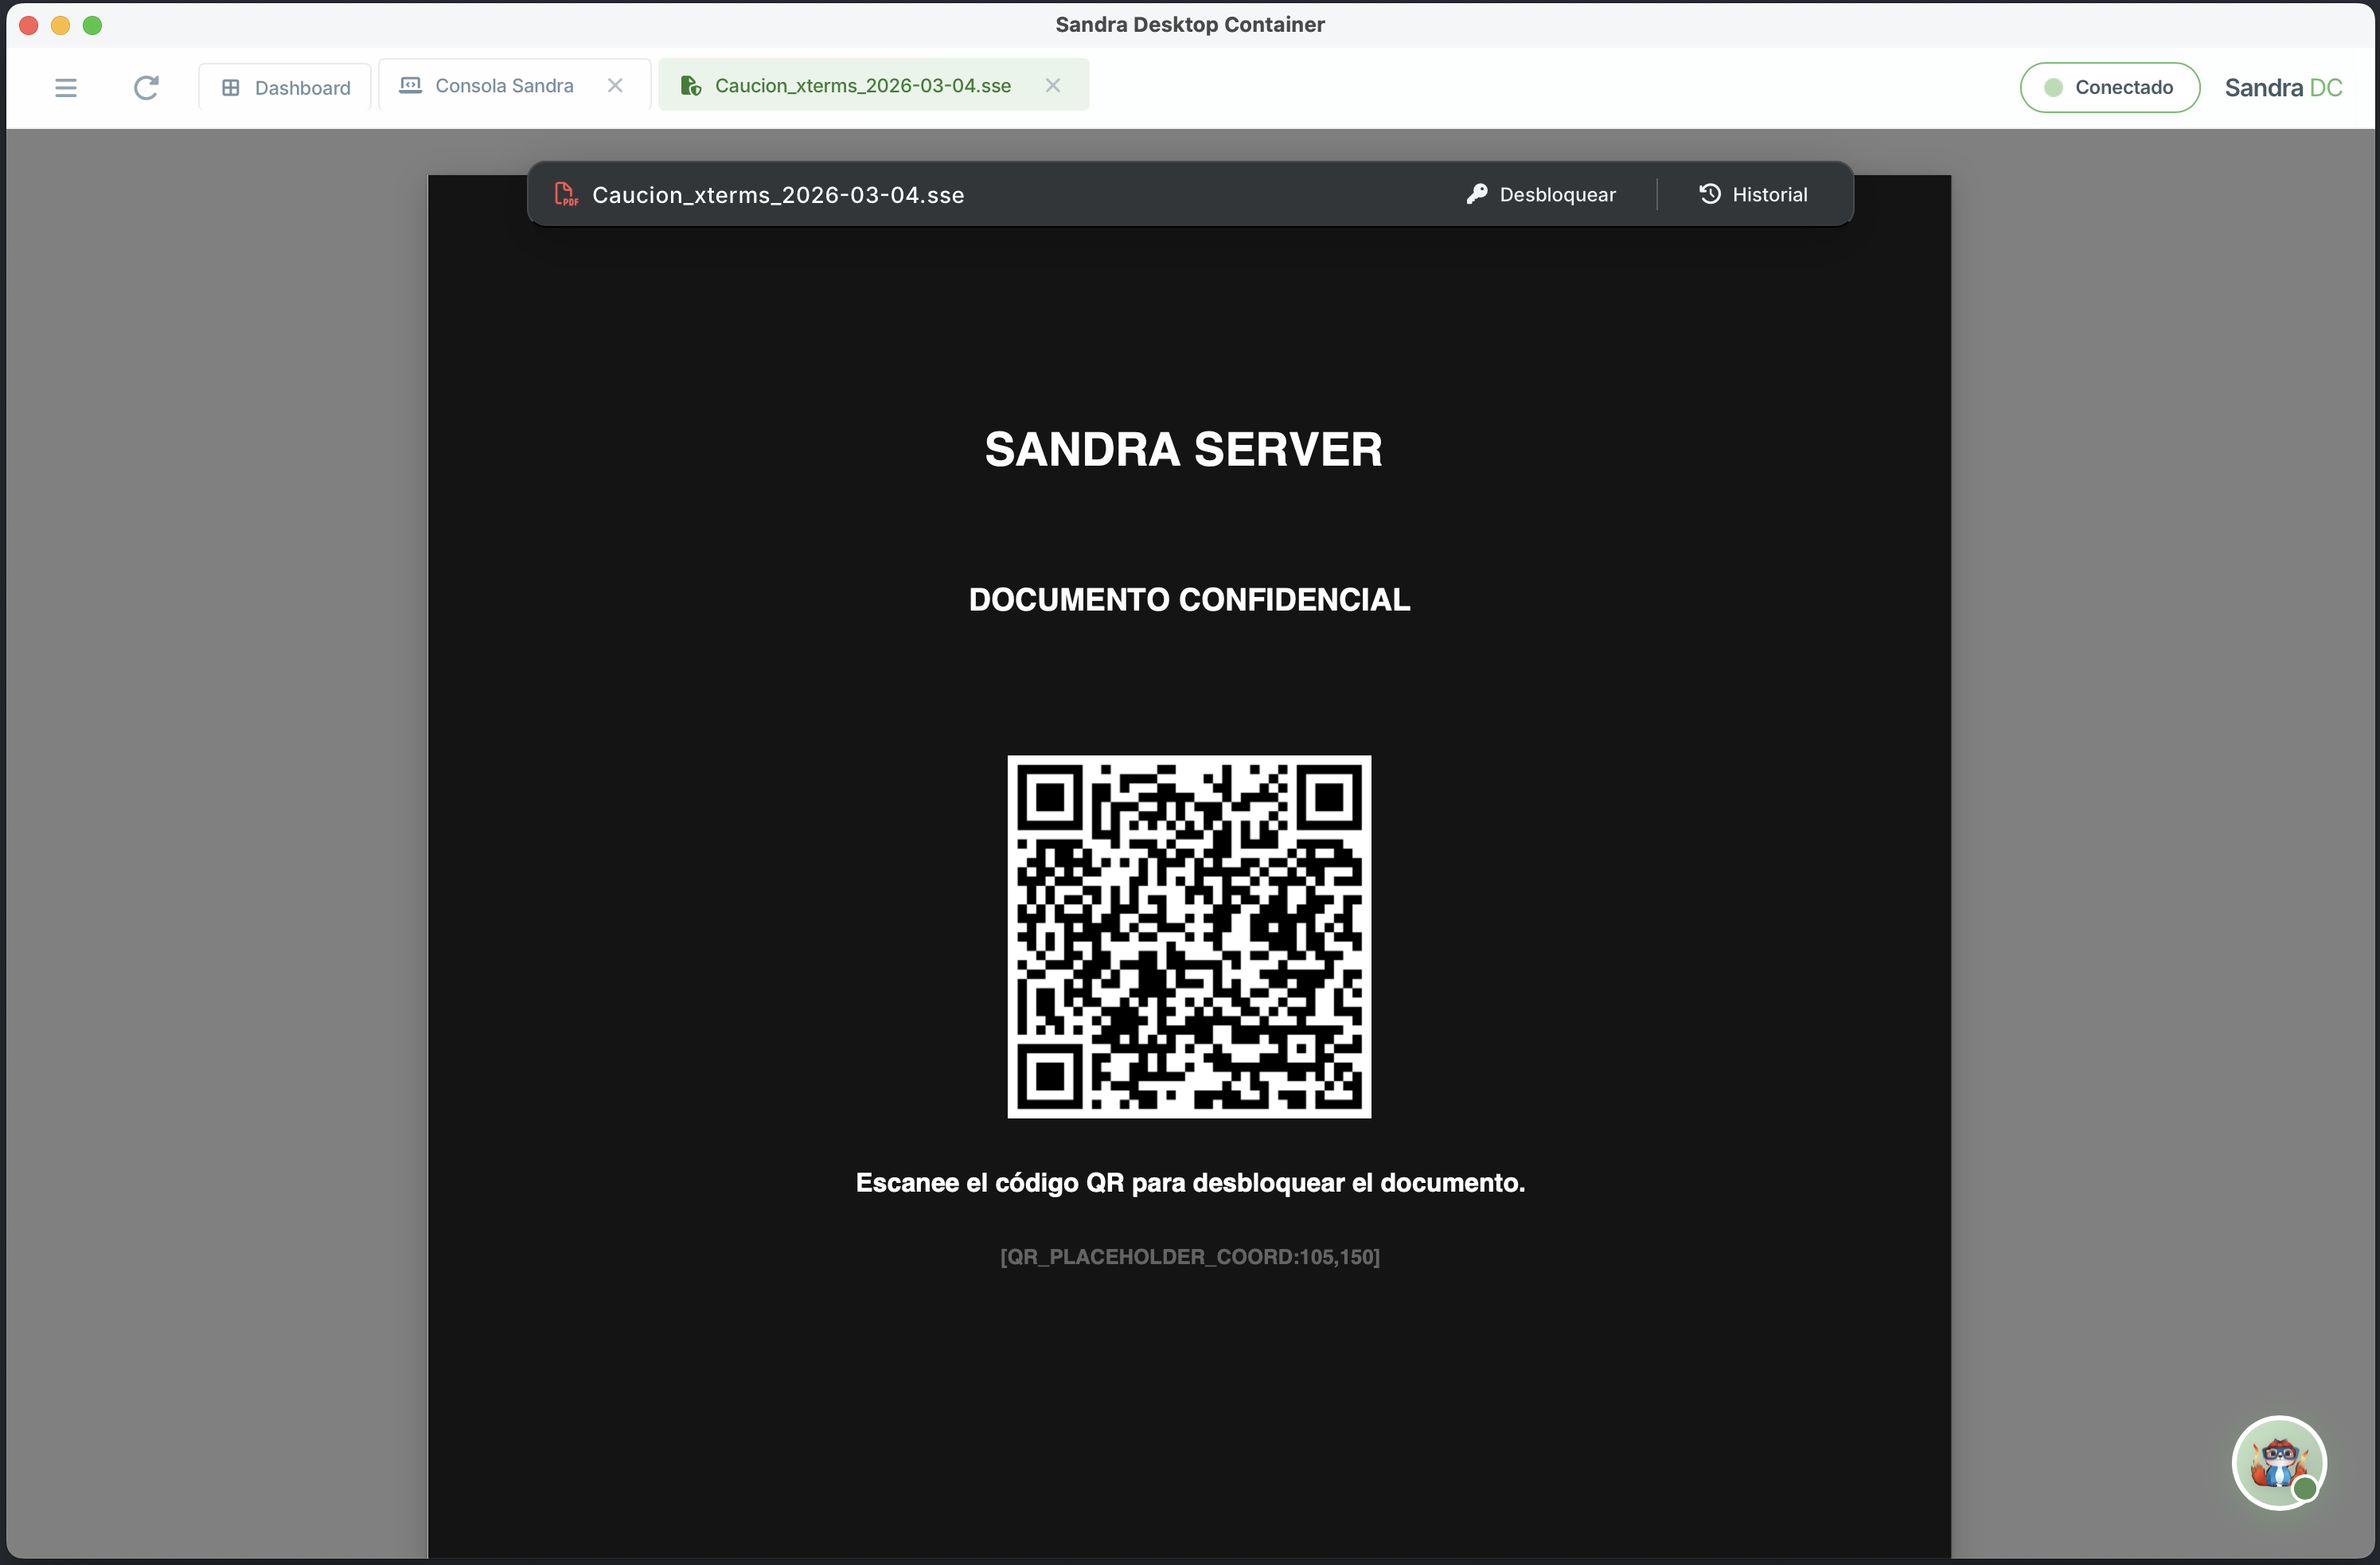
\includegraphics[width=0.95\textwidth]{anexos/12 preview-confidencial.png}
\caption{Vista previa de documento protegido}
\label{fig:preview-protegido}
\end{figure}

Cuando un documento esta protegido, la previsualizacion muestra:

\begin{itemize}[leftmargin=*]
    \item Miniatura de baja resolucion de la primera pagina
    \item Metadatos del archivo (tamano, fecha, autor)
    \item Nivel de clasificacion y etiquetas de seguridad
    \item Indicador de encriptacion activa
    \item Requisitos de acceso (clave, permisos, etc.)
\end{itemize}

\subsection{Desbloqueo con Clave}

\begin{figure}[H]
\centering
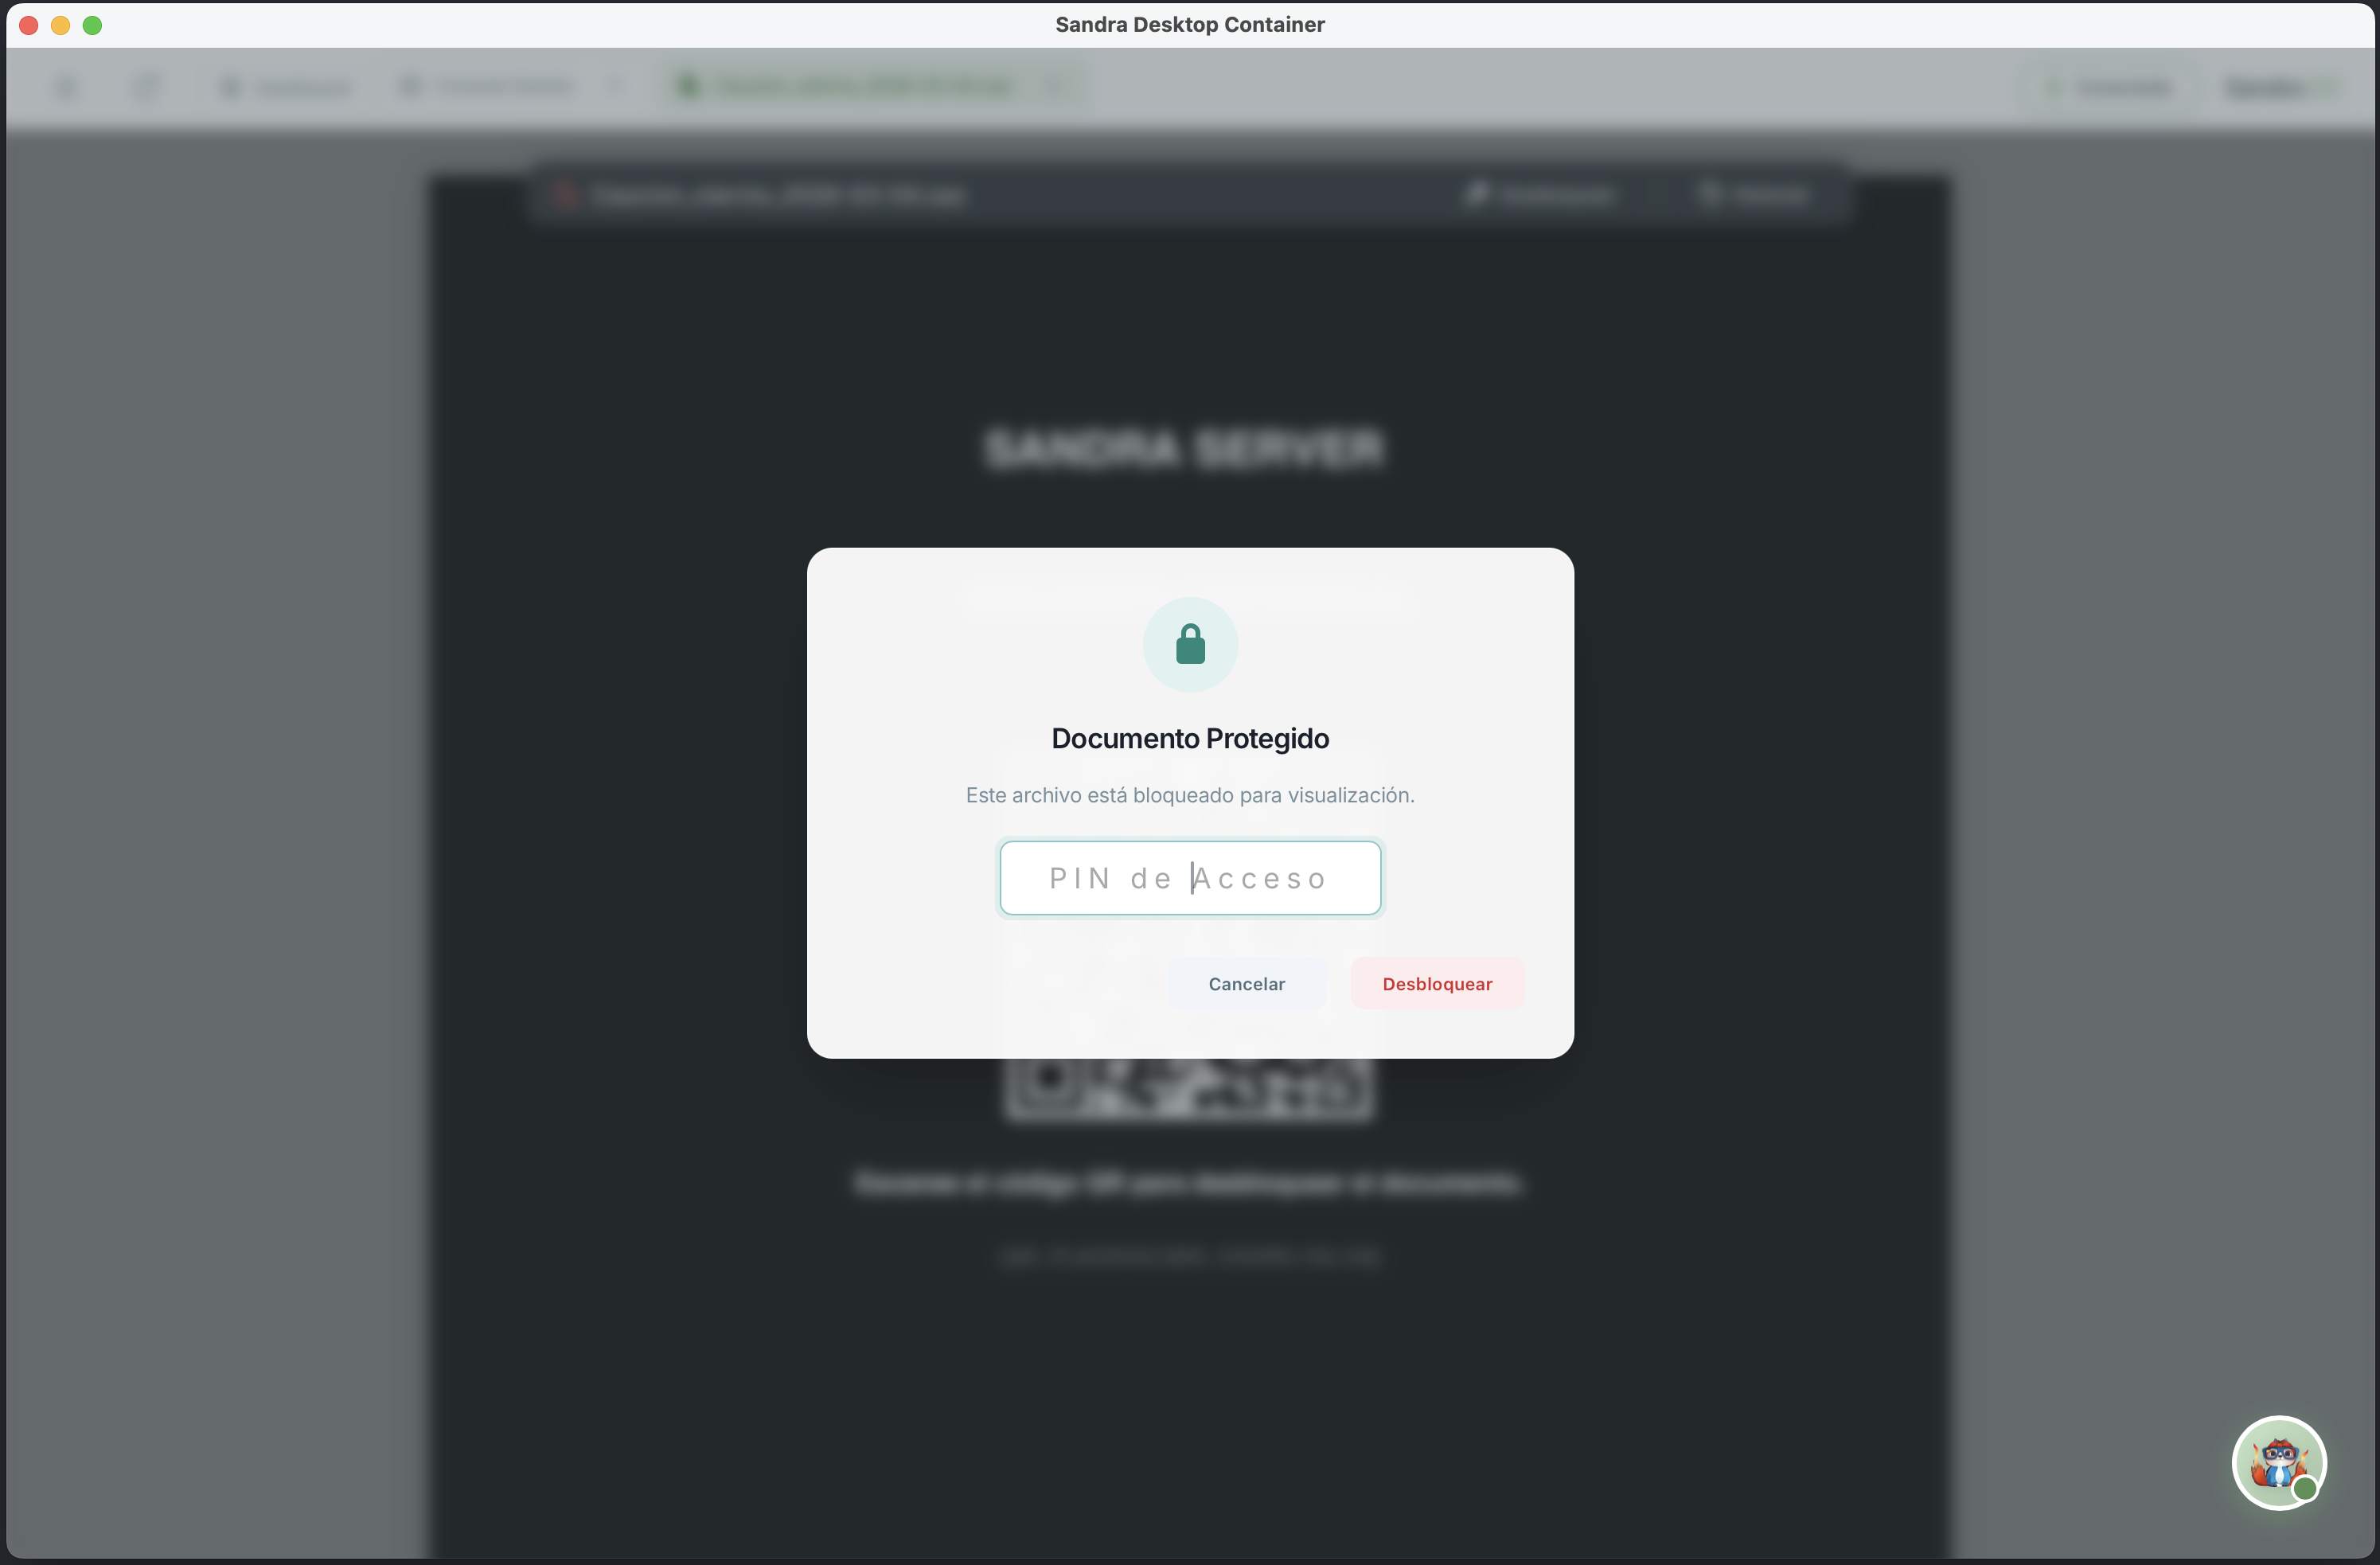
\includegraphics[width=0.95\textwidth]{anexos/12 preview-confidencial-clave.png}
\caption{Panel de autenticacion para desbloqueo}
\label{fig:preview-clave}
\end{figure}

Para acceder al documento completo, el usuario debe:

\begin{enumerate}[leftmargin=*]
    \item Ingresar la clave de desencriptacion o passphrase
    \item Proporcionar credenciales de autenticacion (si aplica)
    \item Confirmar su identidad mediante Client ID
    \item Aceptar los terminos de confidencialidad
\end{enumerate}

\subsection{Vista Desbloqueada}

\begin{figure}[H]
\centering
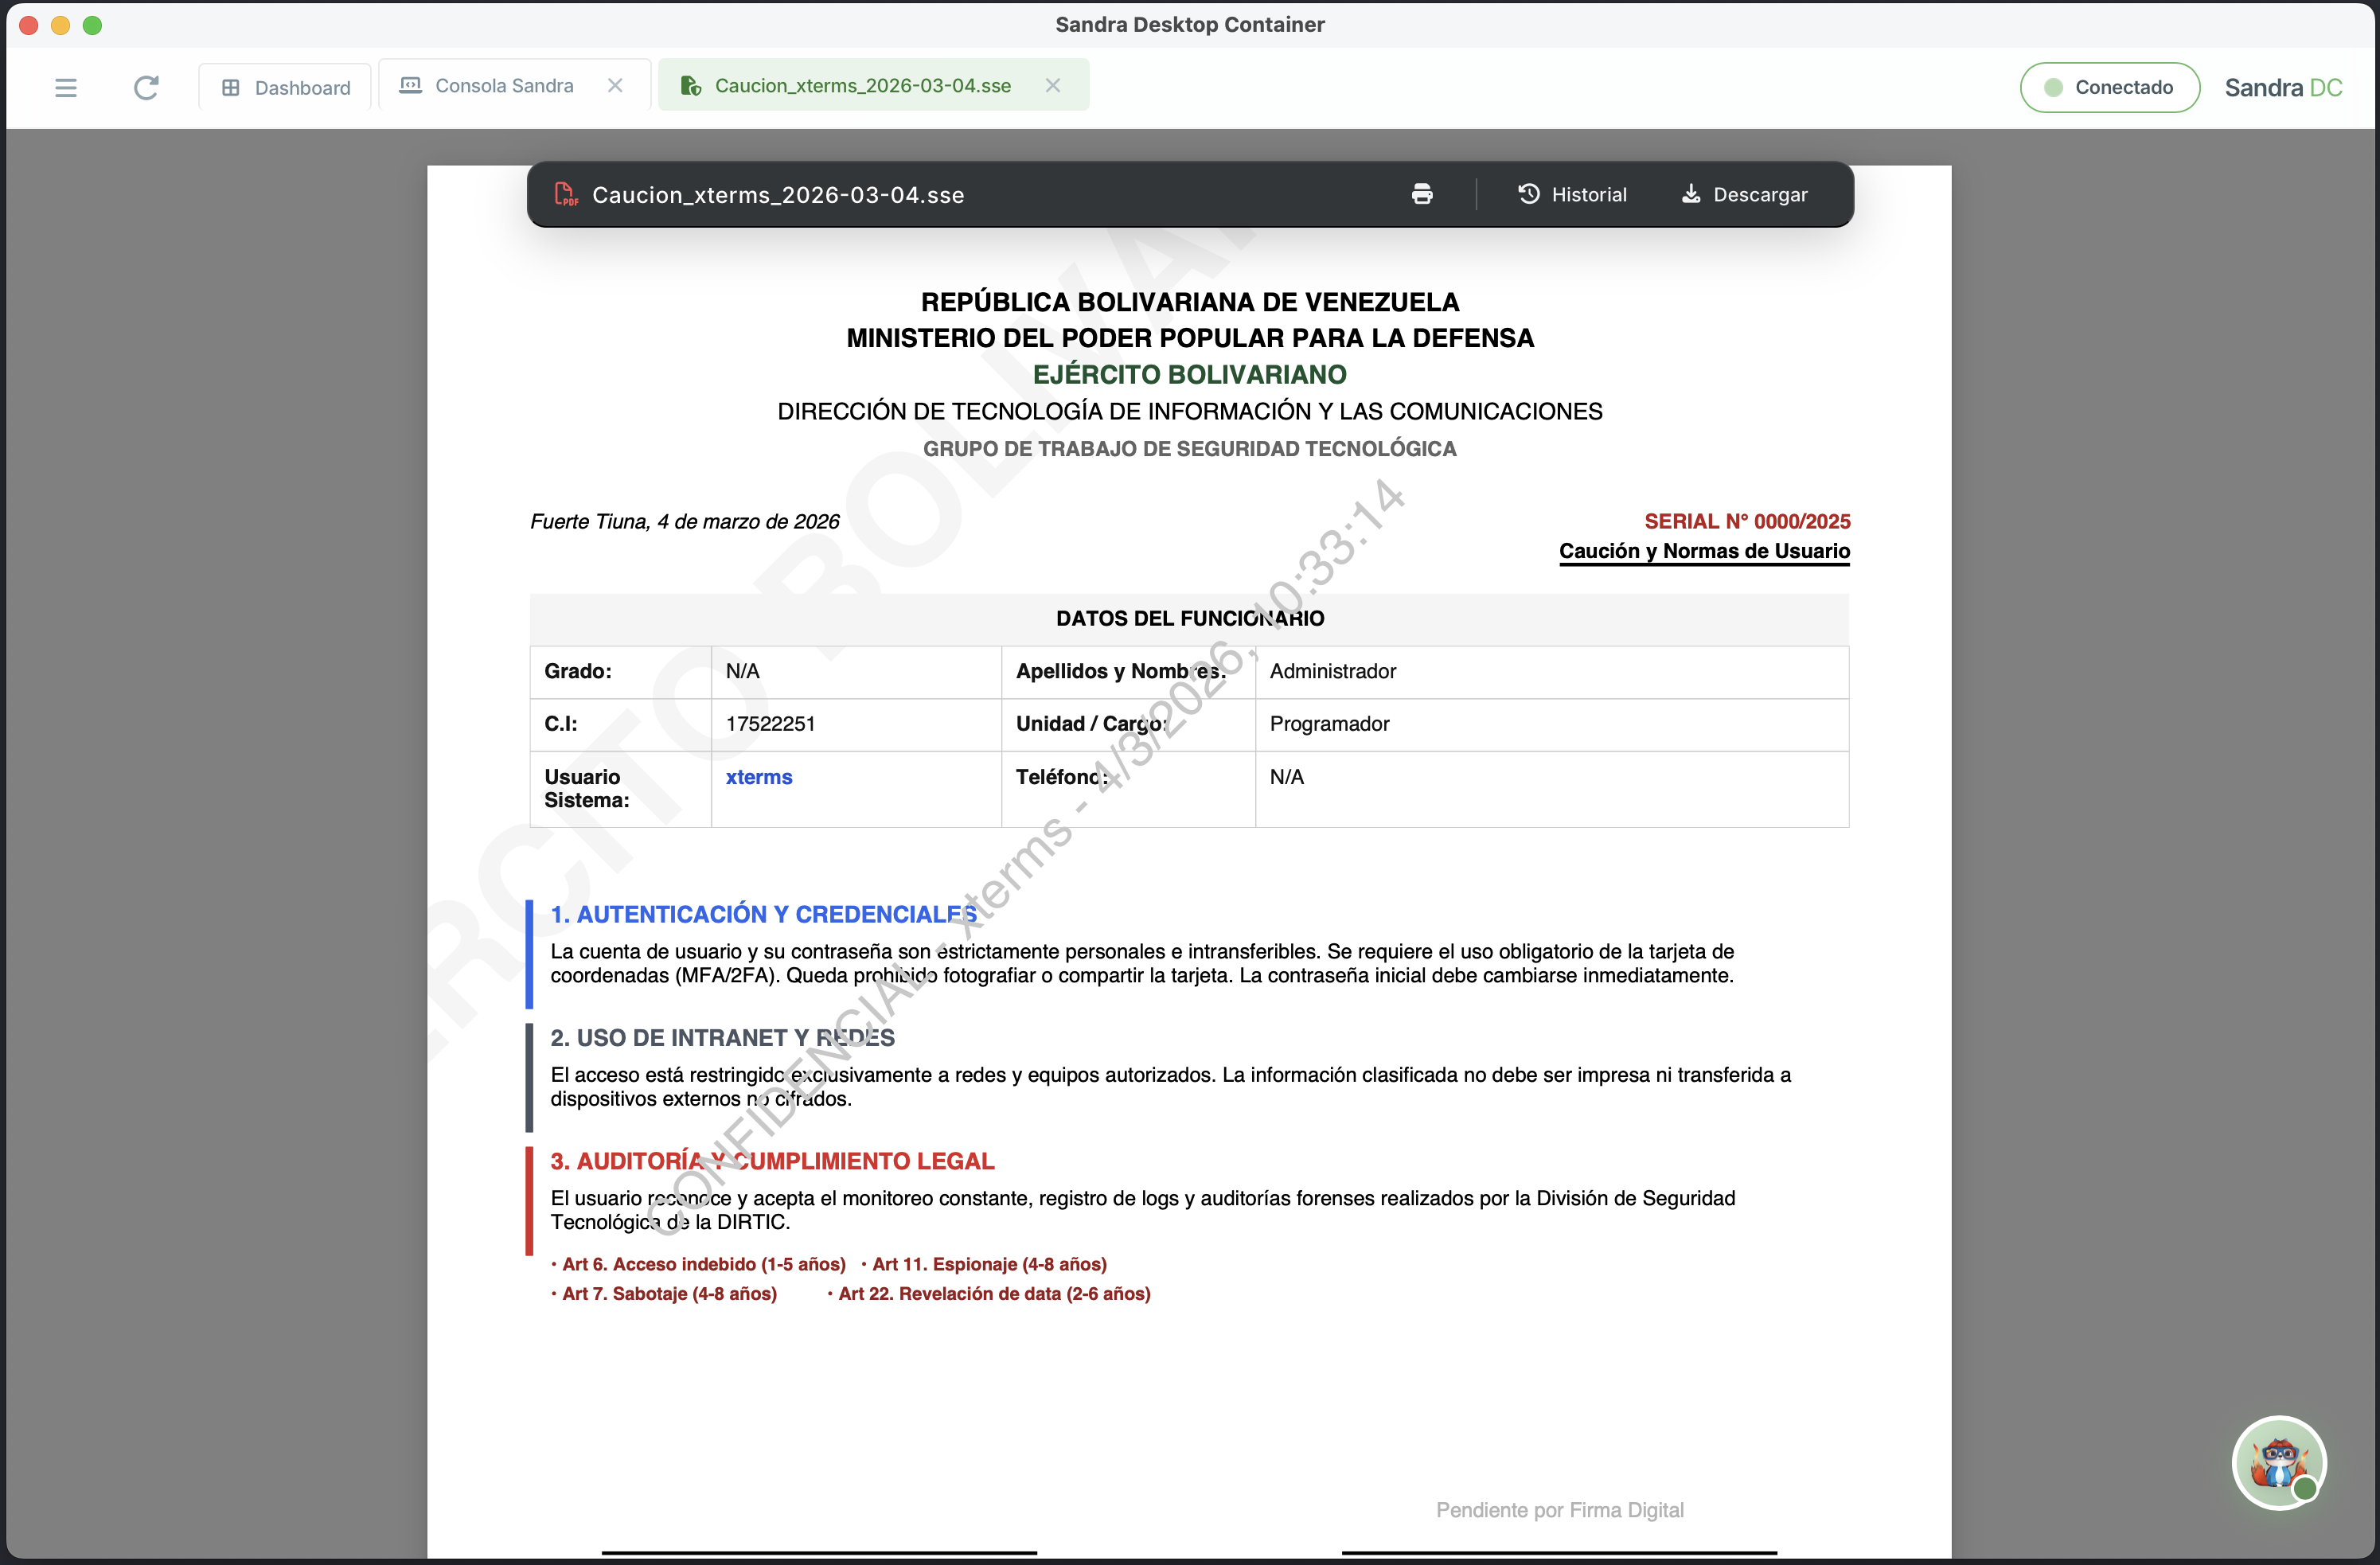
\includegraphics[width=0.95\textwidth]{anexos/12 preview-confidencial-desbloqueado.png}
\caption{Documento en vista completa desbloqueada}
\label{fig:preview-desbloqueado}
\end{figure}

Una vez desbloqueado, el documento se muestra con:

\begin{itemize}[leftmargin=*]
    \item Resolucion completa y nitidez total
    \item Funciones de zoom, rotacion y navegacion
    \item Capacidad de busqueda dentro del documento
    \item Opciones de anotacion (si estan habilitadas)
    \item Marcas de agua dinamicas con identificacion de sesion
\end{itemize}

\begin{quote}
\textbf{Tiempo de Acceso}\\
El acceso desbloqueado es temporal. El documento se bloquea automaticamente:
\begin{itemize}
    \item Al cerrar el visor
    \item Despues del tiempo de inactividad configurado
    \item Al bloquear la pantalla del sistema
    \item Manualmente mediante el boton de bloqueo
\end{itemize}
\end{quote}

\section{Configurador del Visor}
\label{sec:configurador}

El configurador permite ajustar el comportamiento del visor segun las necesidades de seguridad.

\begin{figure}[H]
\centering
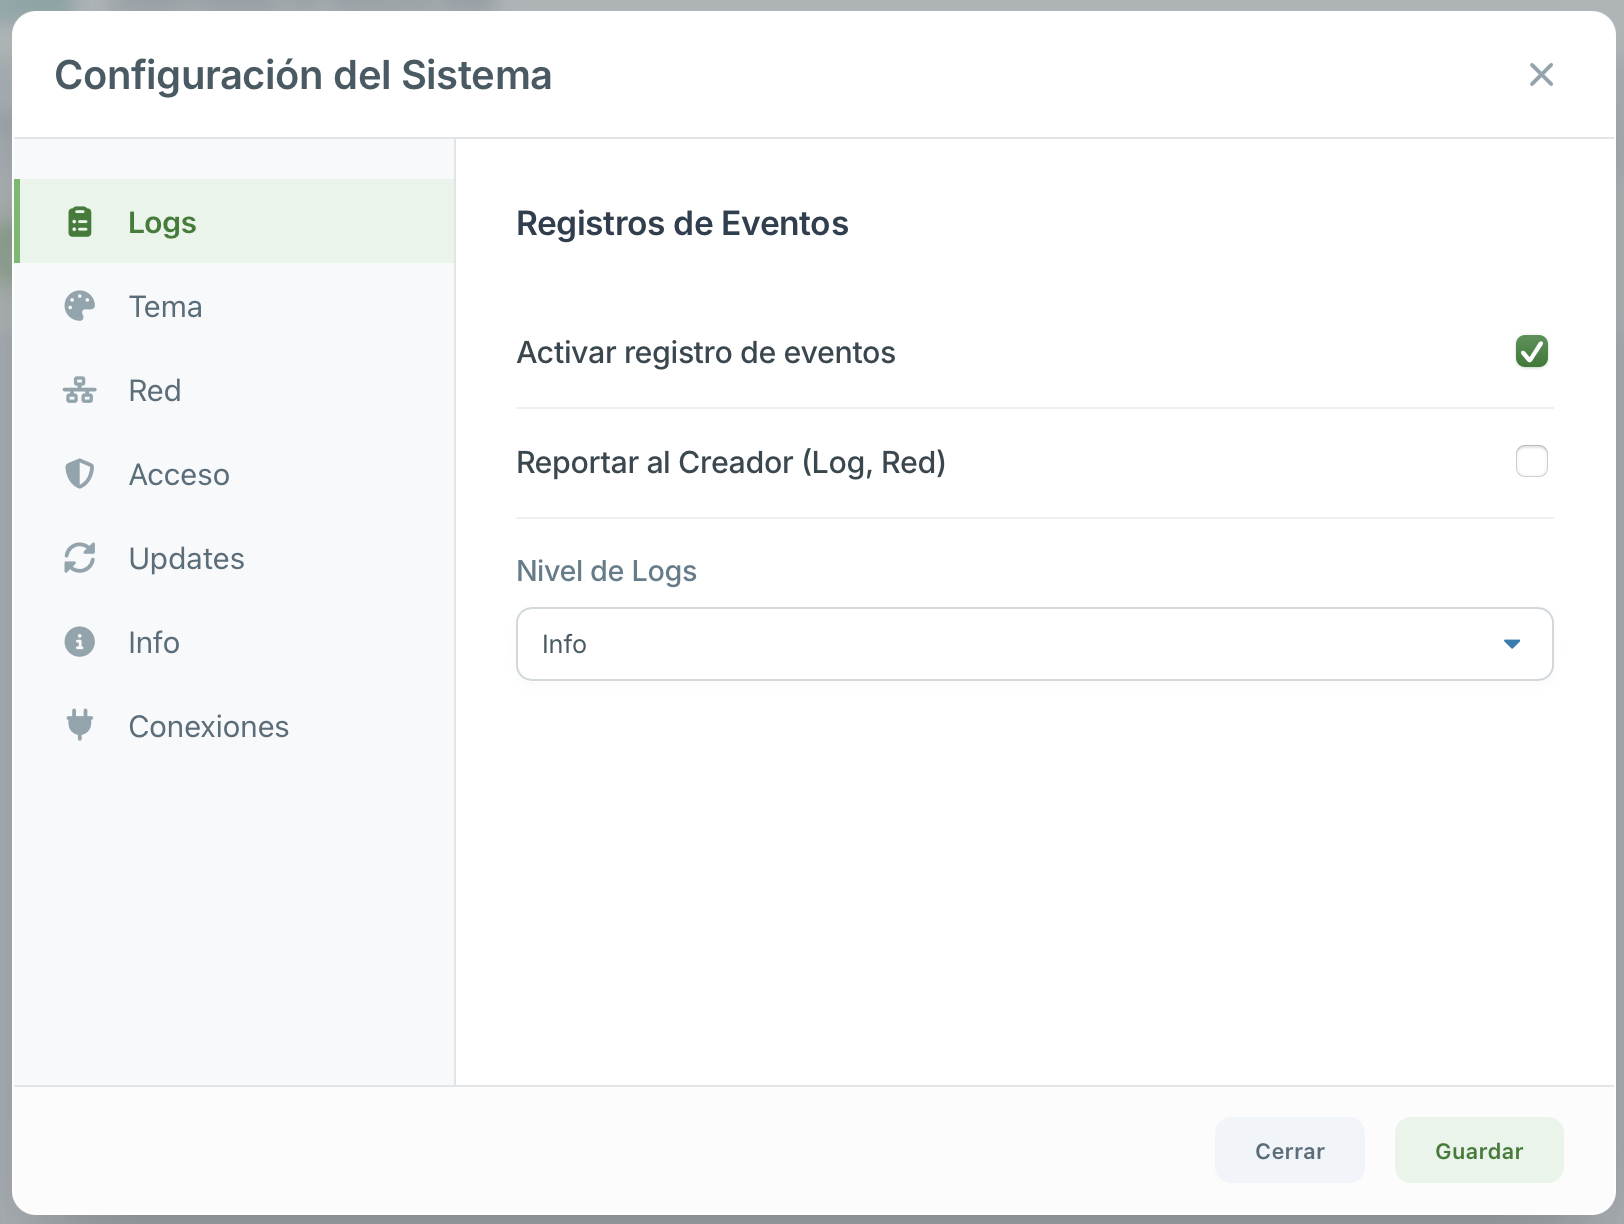
\includegraphics[width=0.95\textwidth]{anexos/15 configurador.png}
\caption{Configurador del visor de documentos}
\label{fig:configurador}
\end{figure}

\subsection{Opciones de Configuracion}

\begin{table}[H]
\centering
\begin{tabular}{p{5cm}p{3cm}p{5cm}}
\toprule
\textbf{Opcion} & \textbf{Valores} & \textbf{Efecto} \\
\midrule
Auto-cierre por inactividad & 1-60 minutos & Cierra documento tras inactividad \\
\midrule
Prevenir capturas de pantalla & Si / No & Bloquea PrintScreen y grabacion \\
\midrule
Marcas de agua dinamicas & Si / No & Superpone ID de sesion en vista \\
\midrule
Nivel de zoom por defecto & 50-200 por ciento & Ajuste inicial de visualizacion \\
\bottomrule
\end{tabular}
\caption{Opciones de configuracion del visor}
\label{tab:config-visor}
\end{table}

\begin{quote}
\textbf{Marcas de Agua Dinamicas}\\
Cuando estan activadas, el visor superpone una marca de agua semitransparente que incluye: Client ID del nodo, timestamp de apertura, y nombre de usuario.
\end{quote}

\section{Flujo de Seguridad del Visor}

El proceso de seguridad del visor sigue estos pasos:

\begin{enumerate}
    \item \textbf{Solicitud de Apertura}: El usuario solicita abrir un documento
    \item \textbf{Autorizacion}: Verificacion de permisos y credenciales
    \item \textbf{Descifrado en RAM}: El documento se descifra en memoria volatil
    \item \textbf{Renderizado}: Visualizacion del contenido descifrado
    \item \textbf{Visualizacion Activa}: El usuario interactua con el documento
    \item \textbf{Cierre}: Al cerrar, se aplica zero-fill a la memoria
    \item \textbf{Registro de Auditoria}: Se registra el evento de acceso
\end{enumerate}

\section{Mejores Practicas}

\begin{enumerate}[leftmargin=*]
    \item Cierra siempre el visor cuando termines de trabajar con documentos sensibles
    \item Habilita el auto-cierre por inactividad (recomendado: 5 minutos)
    \item Usa marcas de agua en entornos compartidos
    \item Bloquea capturas de pantalla para documentos altamente confidenciales
    \item Verifica el hash antes de abrir documentos descargados
\end{enumerate}

\begin{quote}
\textbf{Responsabilidad del Usuario}\\
Aunque el visor proporciona proteccion tecnica robusta, la seguridad final depende del comportamiento del usuario: no fotografiar la pantalla con dispositivos externos, no transcribir informacion sensible a otros medios, cerrar sesion al alejarse del equipo.
\end{quote}

\section{Huella Digital y Trazabilidad de Documentos}
\label{sec:huella-digital}

El Visor de Documentos integra el protocolo \keyconcept{Alquimia Invisible} para proporcionar trazabilidad completa de todos los documentos manipulados.

\notacientifica{Chaque documento visualizado o exportado desde el Visor puede incluir un sello invisible de trazabilidad que permite rastrear su origen en caso de filtración.}

\subsection{Sello de Trazabilidad SDC-Seal}

Cuando se exporta un documento desde el Visor, el sistema inyecta automaticamente un sello de trazabilidad:

\begin{caja}{Informacion del Sello}
\begin{itemize}[leftmargin=1.5em, nosep]
\item Identificador del dispositivo emisor
\item Identificador del usuario que realizo la exportacion
\item Timestamp de generacion
\item Hash del contenido original
\end{itemize}
\end{caja}

\notacientifica{El sello utiliza tecnicas de esteganografia avanzada (Zero-Width Bit Encoding) que son completamente invisibles al usuario pero verificables por el sistema.}

\begin{figure}[H]
\centering
\fbox{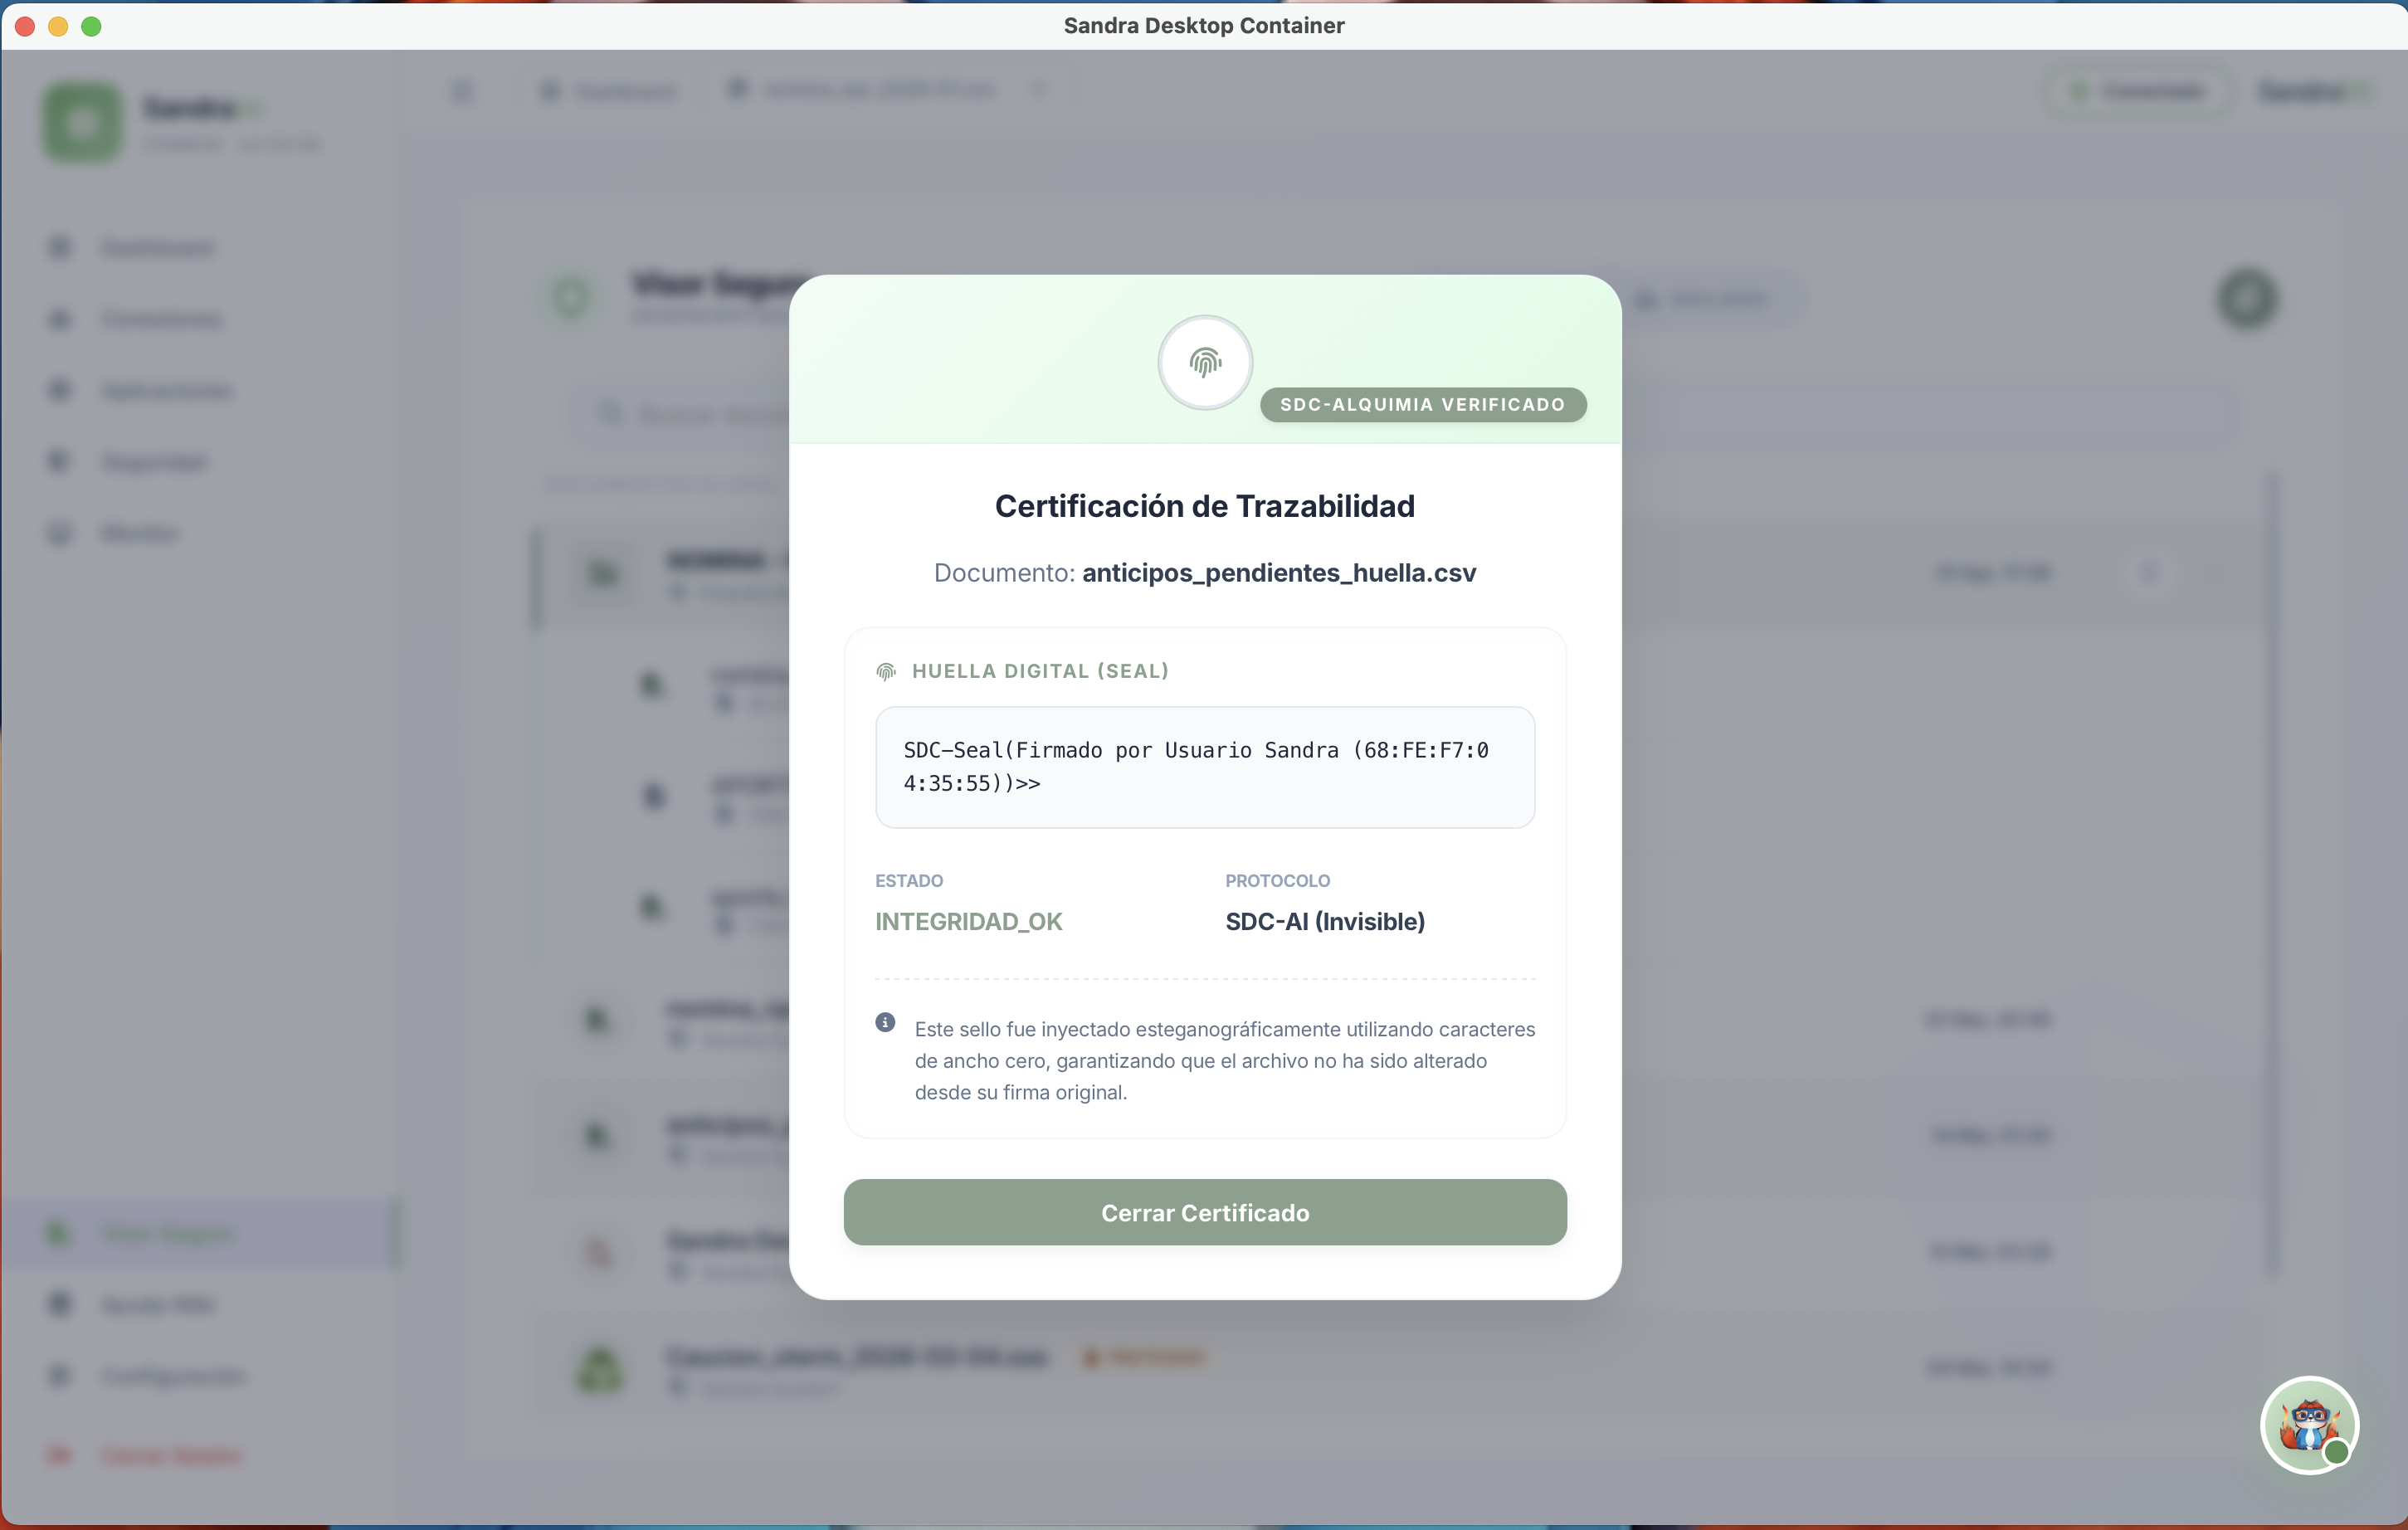
\includegraphics[width=0.7\textwidth]{anexos/11 visor.huelladigital.png}}
\caption{Activacion del sello de trazabilidad en el Visor}
\label{fig:visor-huella}
\end{figure}

\notacientifica{El usuario puede activar o desactivar el sellado desde la interfaz del Visor. Por defecto, el sistema esta configurado para sellar automaticamente todos los documentos exportados.}

\subsection{Huella Digital del Documento}

El Visor muestra la huella digital de cada documento:

\begin{caja}{Informacion de Huella}
\begin{itemize}[leftmargin=1.5em, nosep]
\item \textbf{Hash de contenido}: Identificador unico del contenido
\item \textbf{Estado del sello}: Activo/Inactivo/Invalido
\item \textbf{Fecha de creacion}: Cuando fue generado el documento
\item \textbf{Origen}: Usuario y dispositivo que lo crearon
\item \textbf{Trazabilidad}: Historial de movimientos del documento
\end{itemize}
\end{caja}

\notacientifica{Esta informacion permite al usuario saber instantaneamente si un documento esta protegido por Alquimia Invisible.}

\subsection{Exportacion con Proteccion SSE}

El Visor soporta exportacion con cifrado del lado del servidor (Server-Side Encryption):

\begin{caja}{Opciones de Exportacion Protegida}
\begin{itemize}[leftmargin=1.5em, nosep]
\item \textbf{Exportar SSE}: Cifrado con clave gestionada por SDC
\item \textbf{Exportar GPG}: Cifrado con clave publica GPG
\item \textbf{Exportar SSE + Sello}: Cifrado + trazabilidad invisible
\end{itemize}
\end{caja}

\notacientifica{La combinacion de cifrado y trazabilidad proporciona multiple capas de proteccion para documentos sensibles.}

\begin{figure}[H]
\centering
\fbox{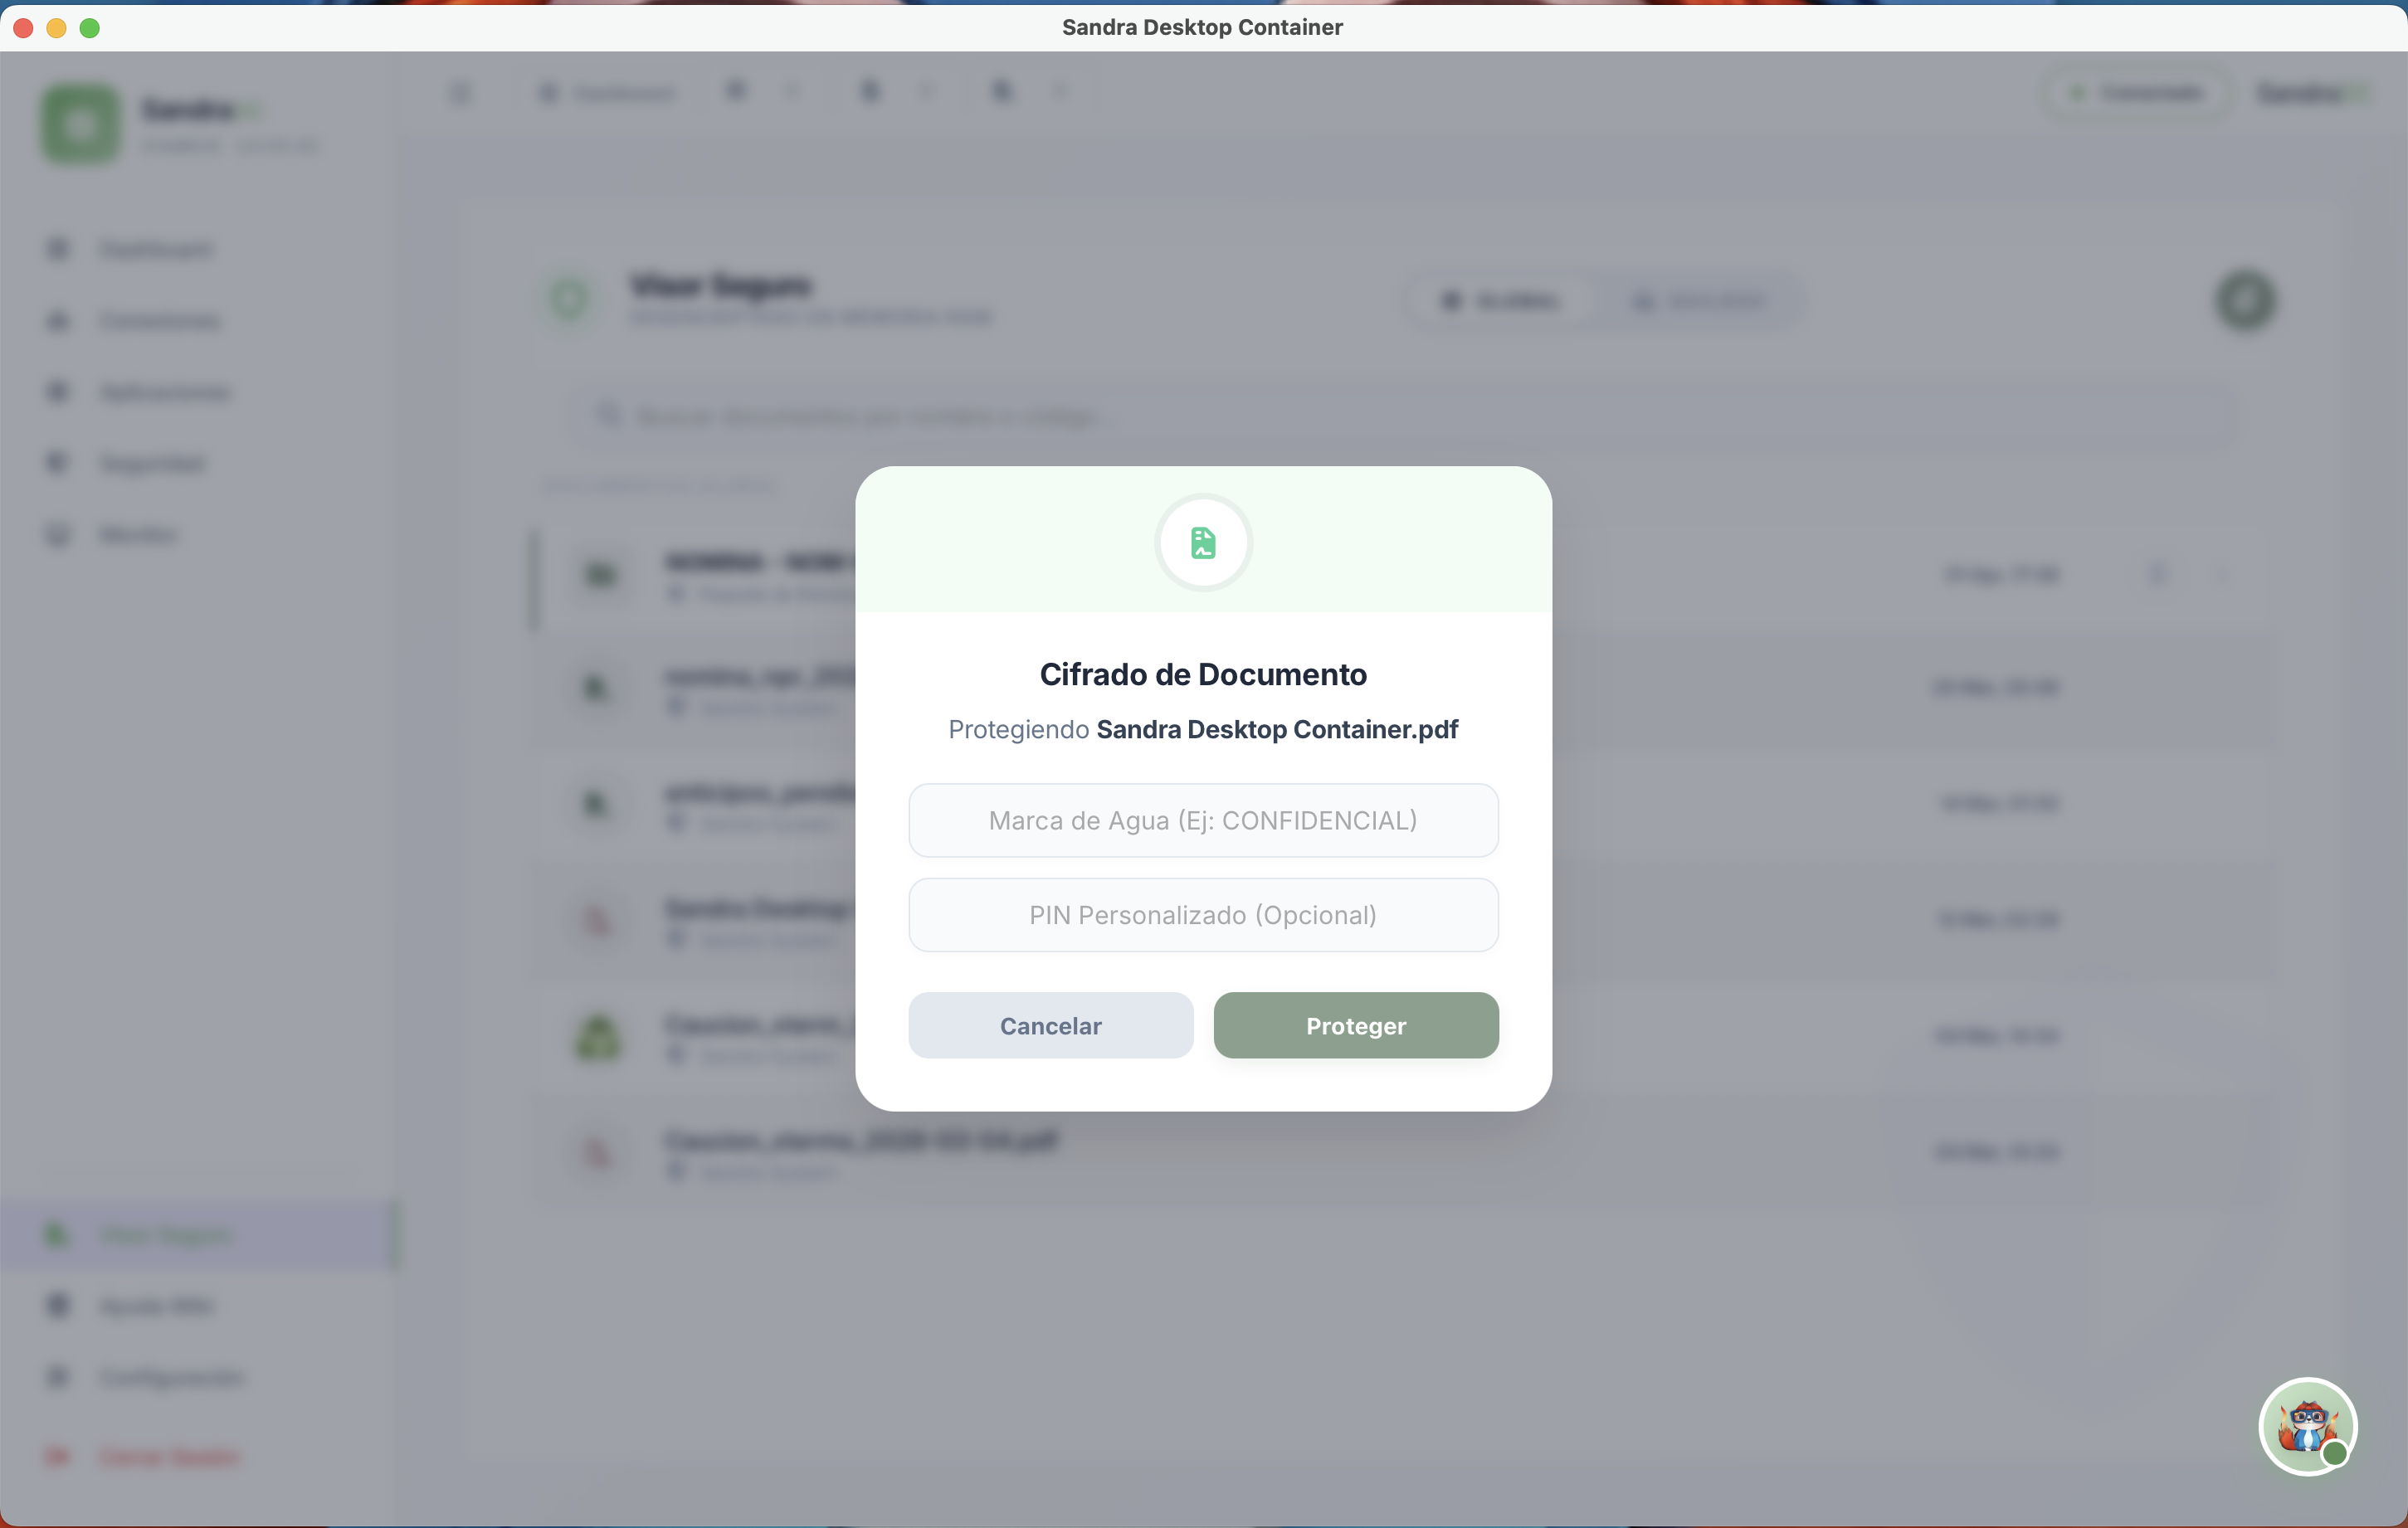
\includegraphics[width=0.65\textwidth]{anexos/11 visor encriptar.png}}
\caption{Opciones de cifrado en exportacion}
\label{fig:visor-encriptar-opts}
\end{figure}

\notacientifica{Para mas detalles sobre el protocolo Alquimia Invisible, consulte el Capitulo 8 de este manual.}

\section{Previsualizacion de Archivos CSV}
\label{sec:preview-csv}

El visor permite previsualizar archivos CSV de forma rapida y eficiente.

\begin{figure}[H]
\centering
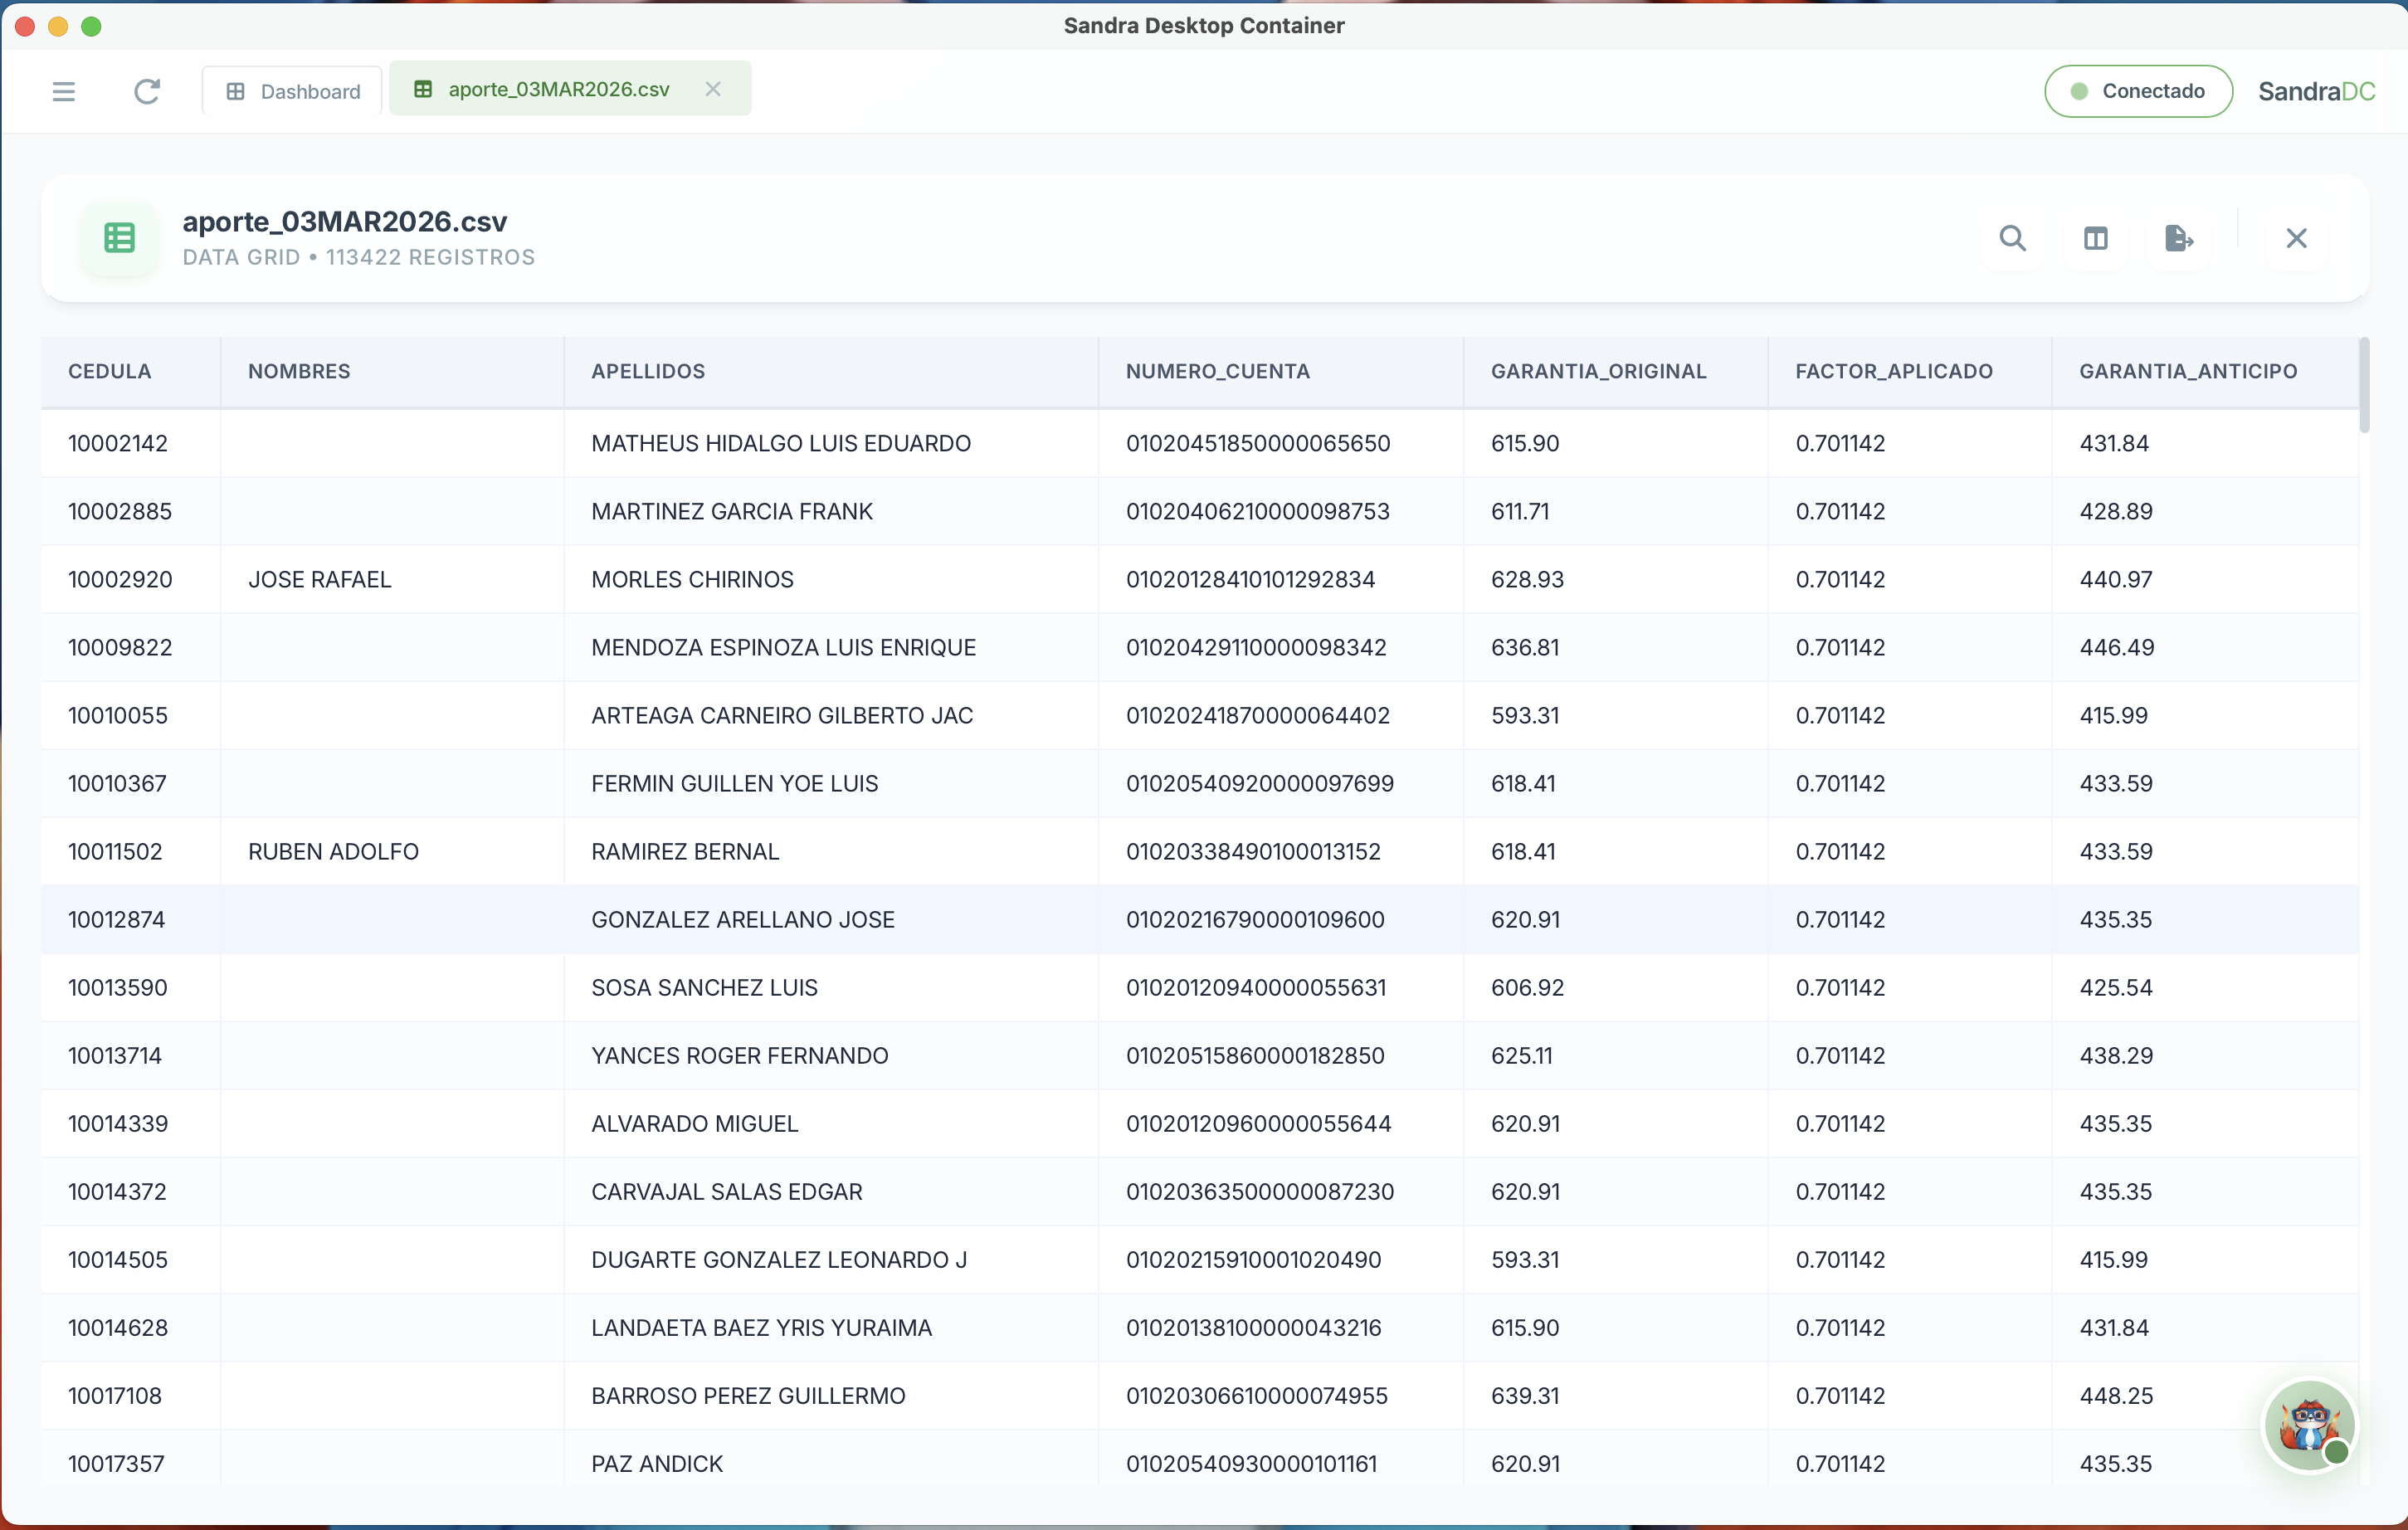
\includegraphics[width=0.65\textwidth]{anexos/12 preview-csv.png}
\caption{Previsualizacion de archivo CSV}
\label{fig:preview-csv}
\end{figure}

\subsection{Filtros y Busqueda}

\begin{figure}[H]
\centering
\fbox{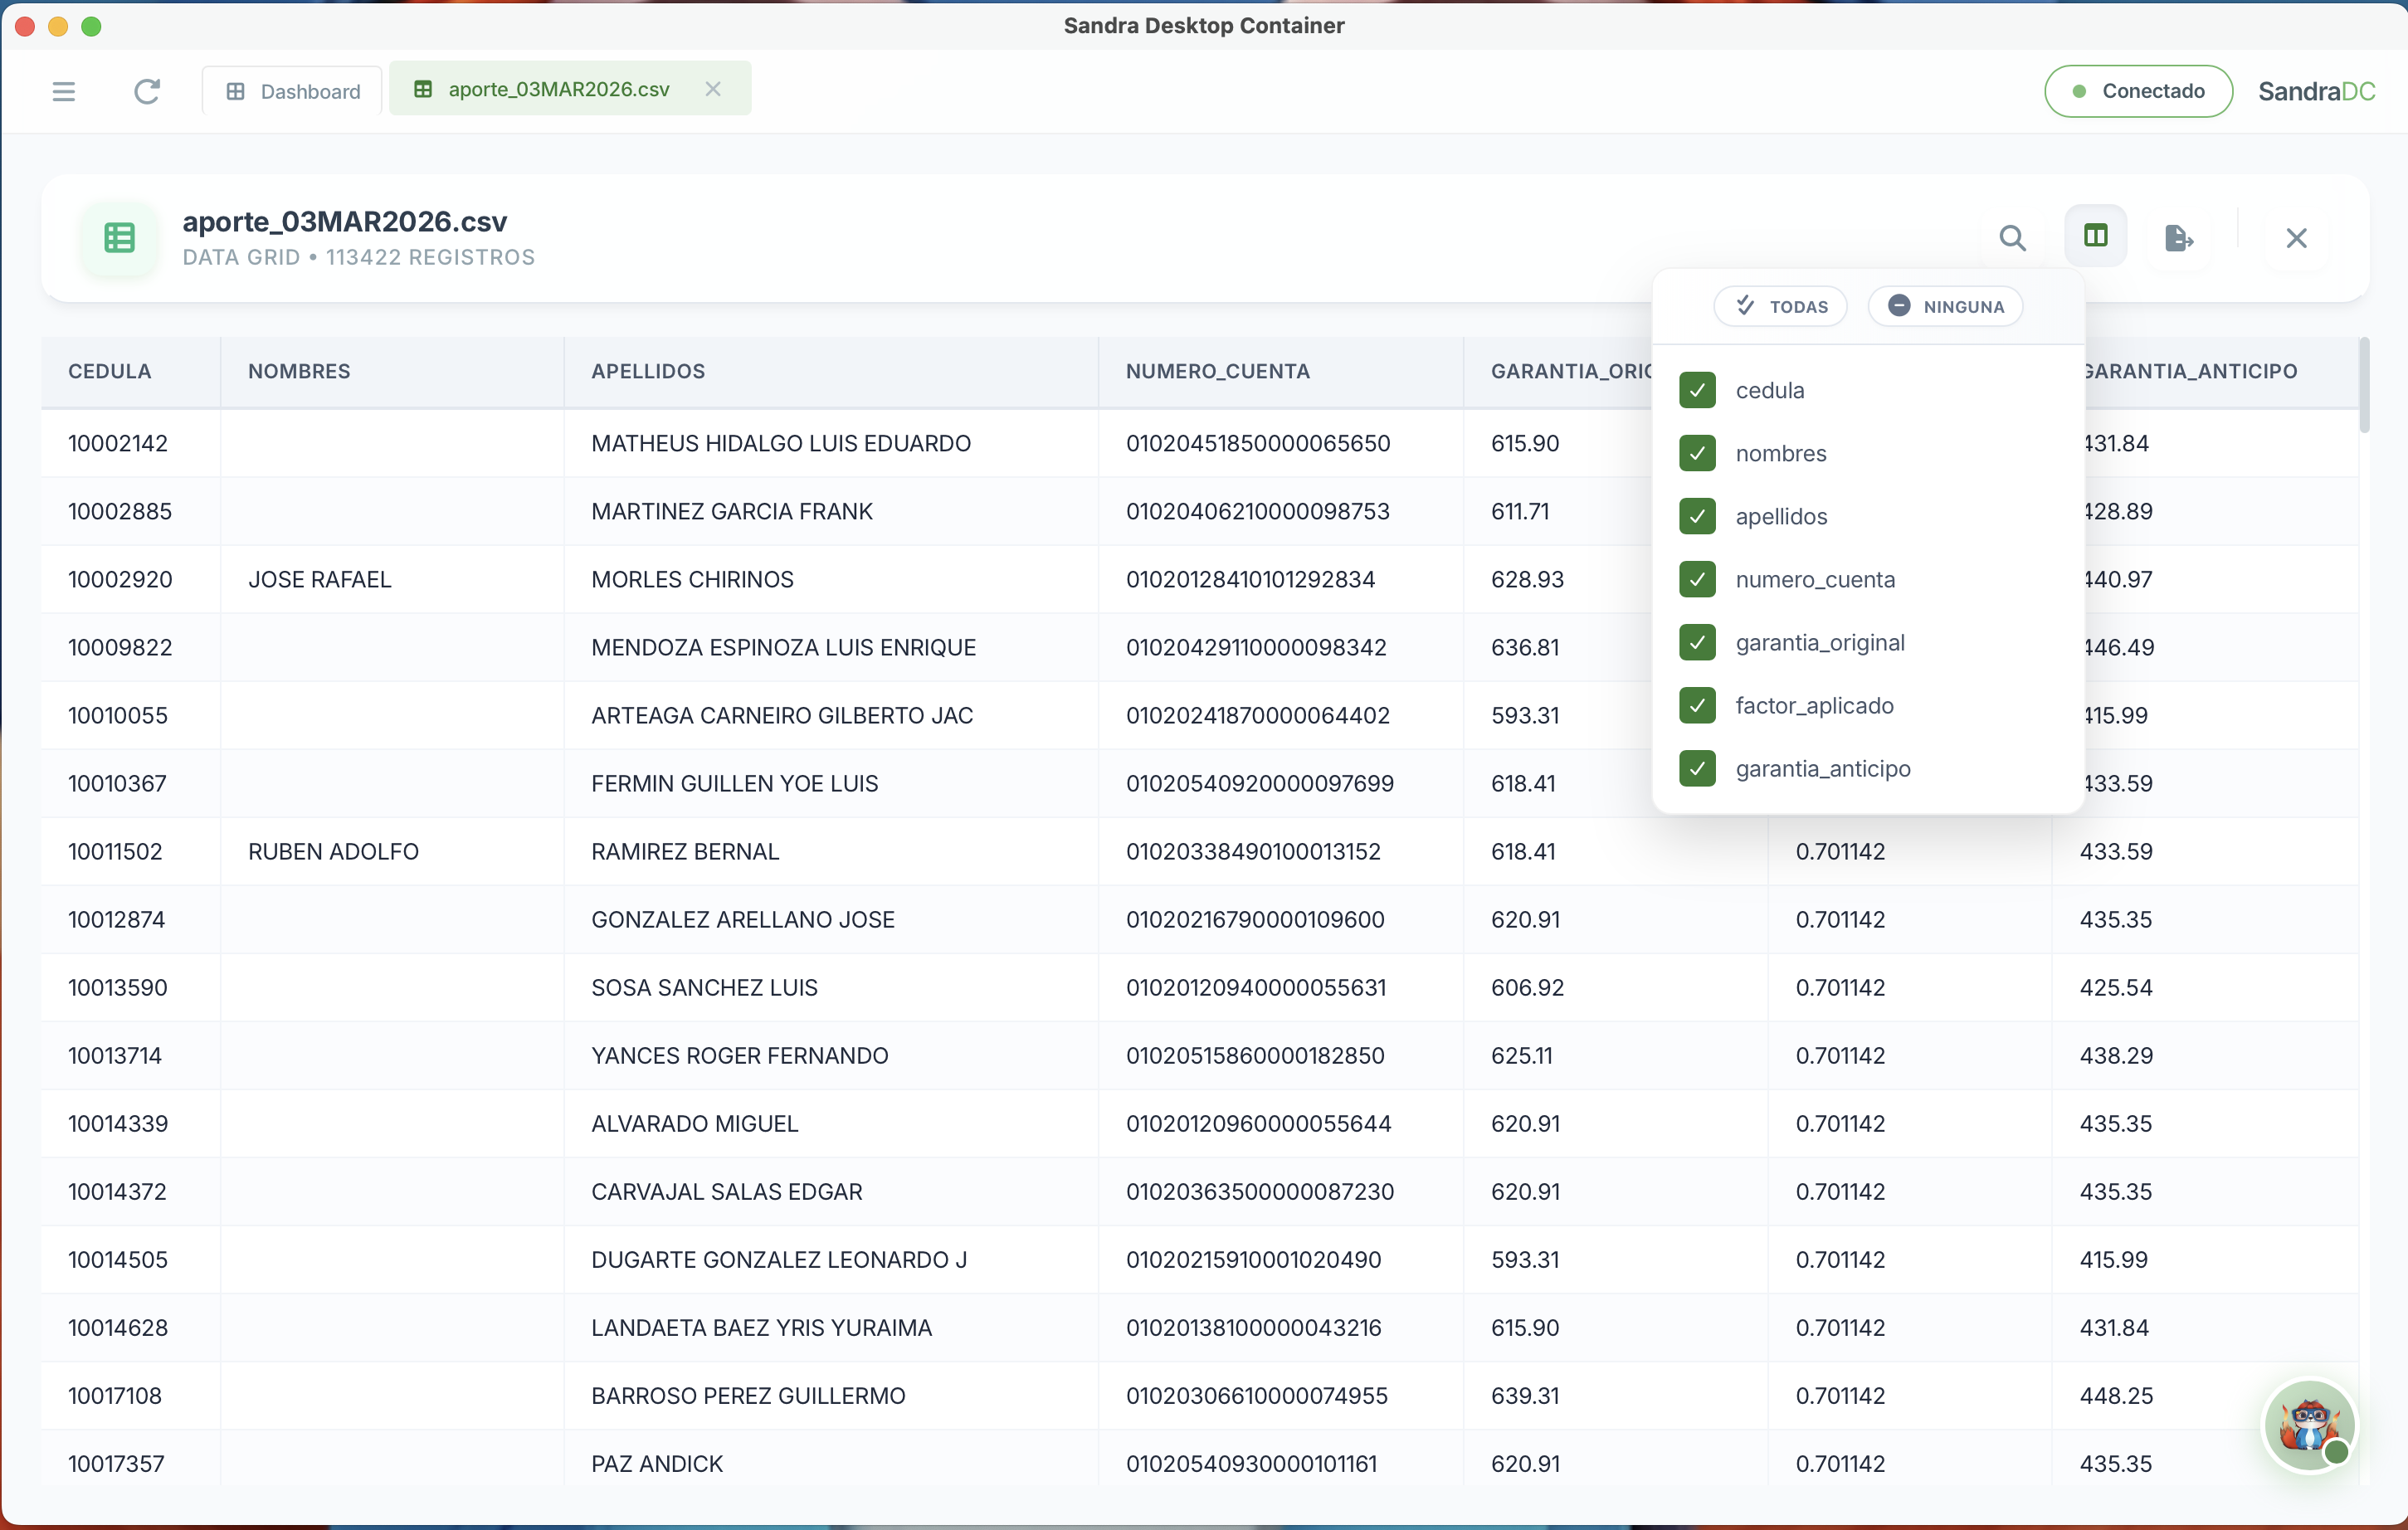
\includegraphics[width=0.65\textwidth]{anexos/12 preview-csv.filtro.png}}
\caption{Filtros disponibles en previsualizacion CSV}
\label{fig:csv-filtro}
\end{figure}

El sistema de previsualizacion CSV permite:

\begin{itemize}[leftmargin=*]
    \item Filtrar columnas por criterios especificos
    \item Buscar valores en tiempo real
    \item Ordenar datos por cualquier columna
    \item Exportar solo la seleccion actual
\end{itemize}

\begin{caja}{Optimizacion de Rendimiento}
Los archivos CSV grandes se previsualizan de forma paginada, cargando solo las primeras 1000 filas para mantener la fluidez de la interfaz. La busqueda opera sobre indices en memoria para respuestas instantaneas.
\end{caja}

\begin{figure}[H]
\centering
\fbox{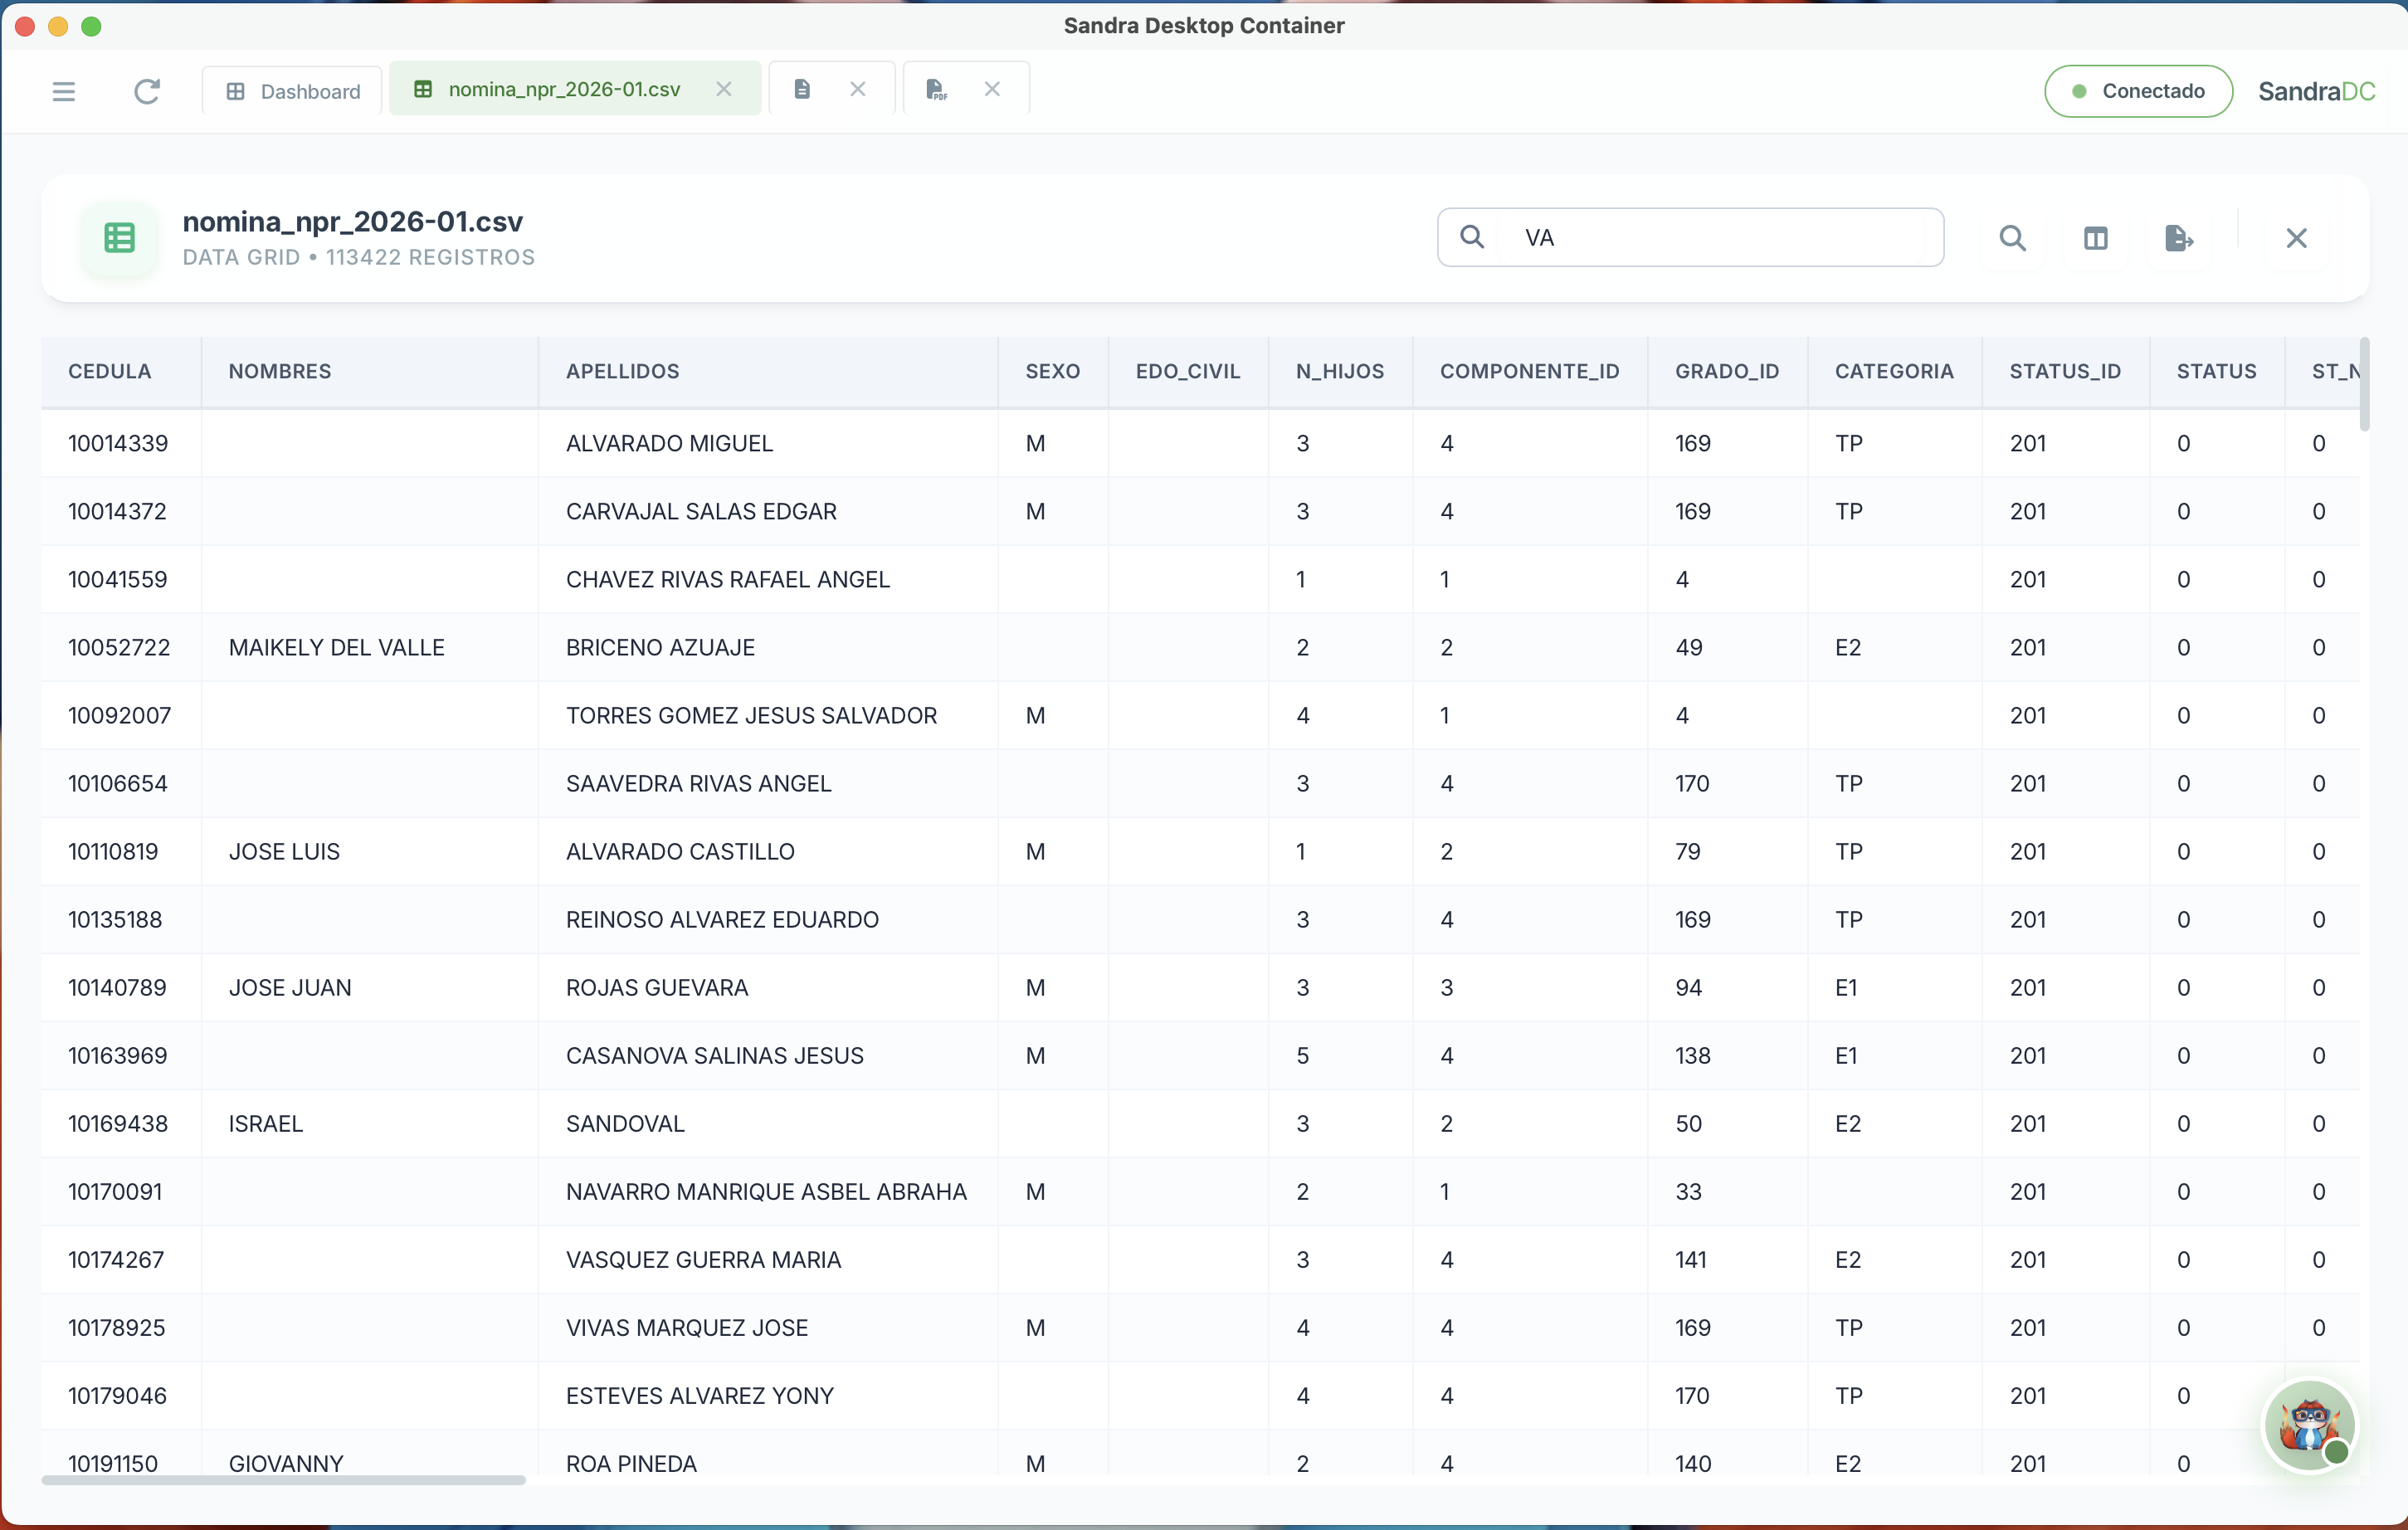
\includegraphics[width=0.65\textwidth]{anexos/12 preview-csv.buscar.png}}
\caption{Barra de busqueda en previsualizacion}
\label{fig:csv-buscar}
\end{figure}

\notacientifica{El visor de CSV soporta codificacion UTF-8 y detecta automaticamente el delimitador (coma, punto y coma, tabulador).}

\section{Eliminacion de Documentos}
\label{sec:eliminar-doc}

El sistema de eliminacion segura garantiza que los documentos borrados no puedan ser recuperados.

\begin{figure}[H]
\centering
\fbox{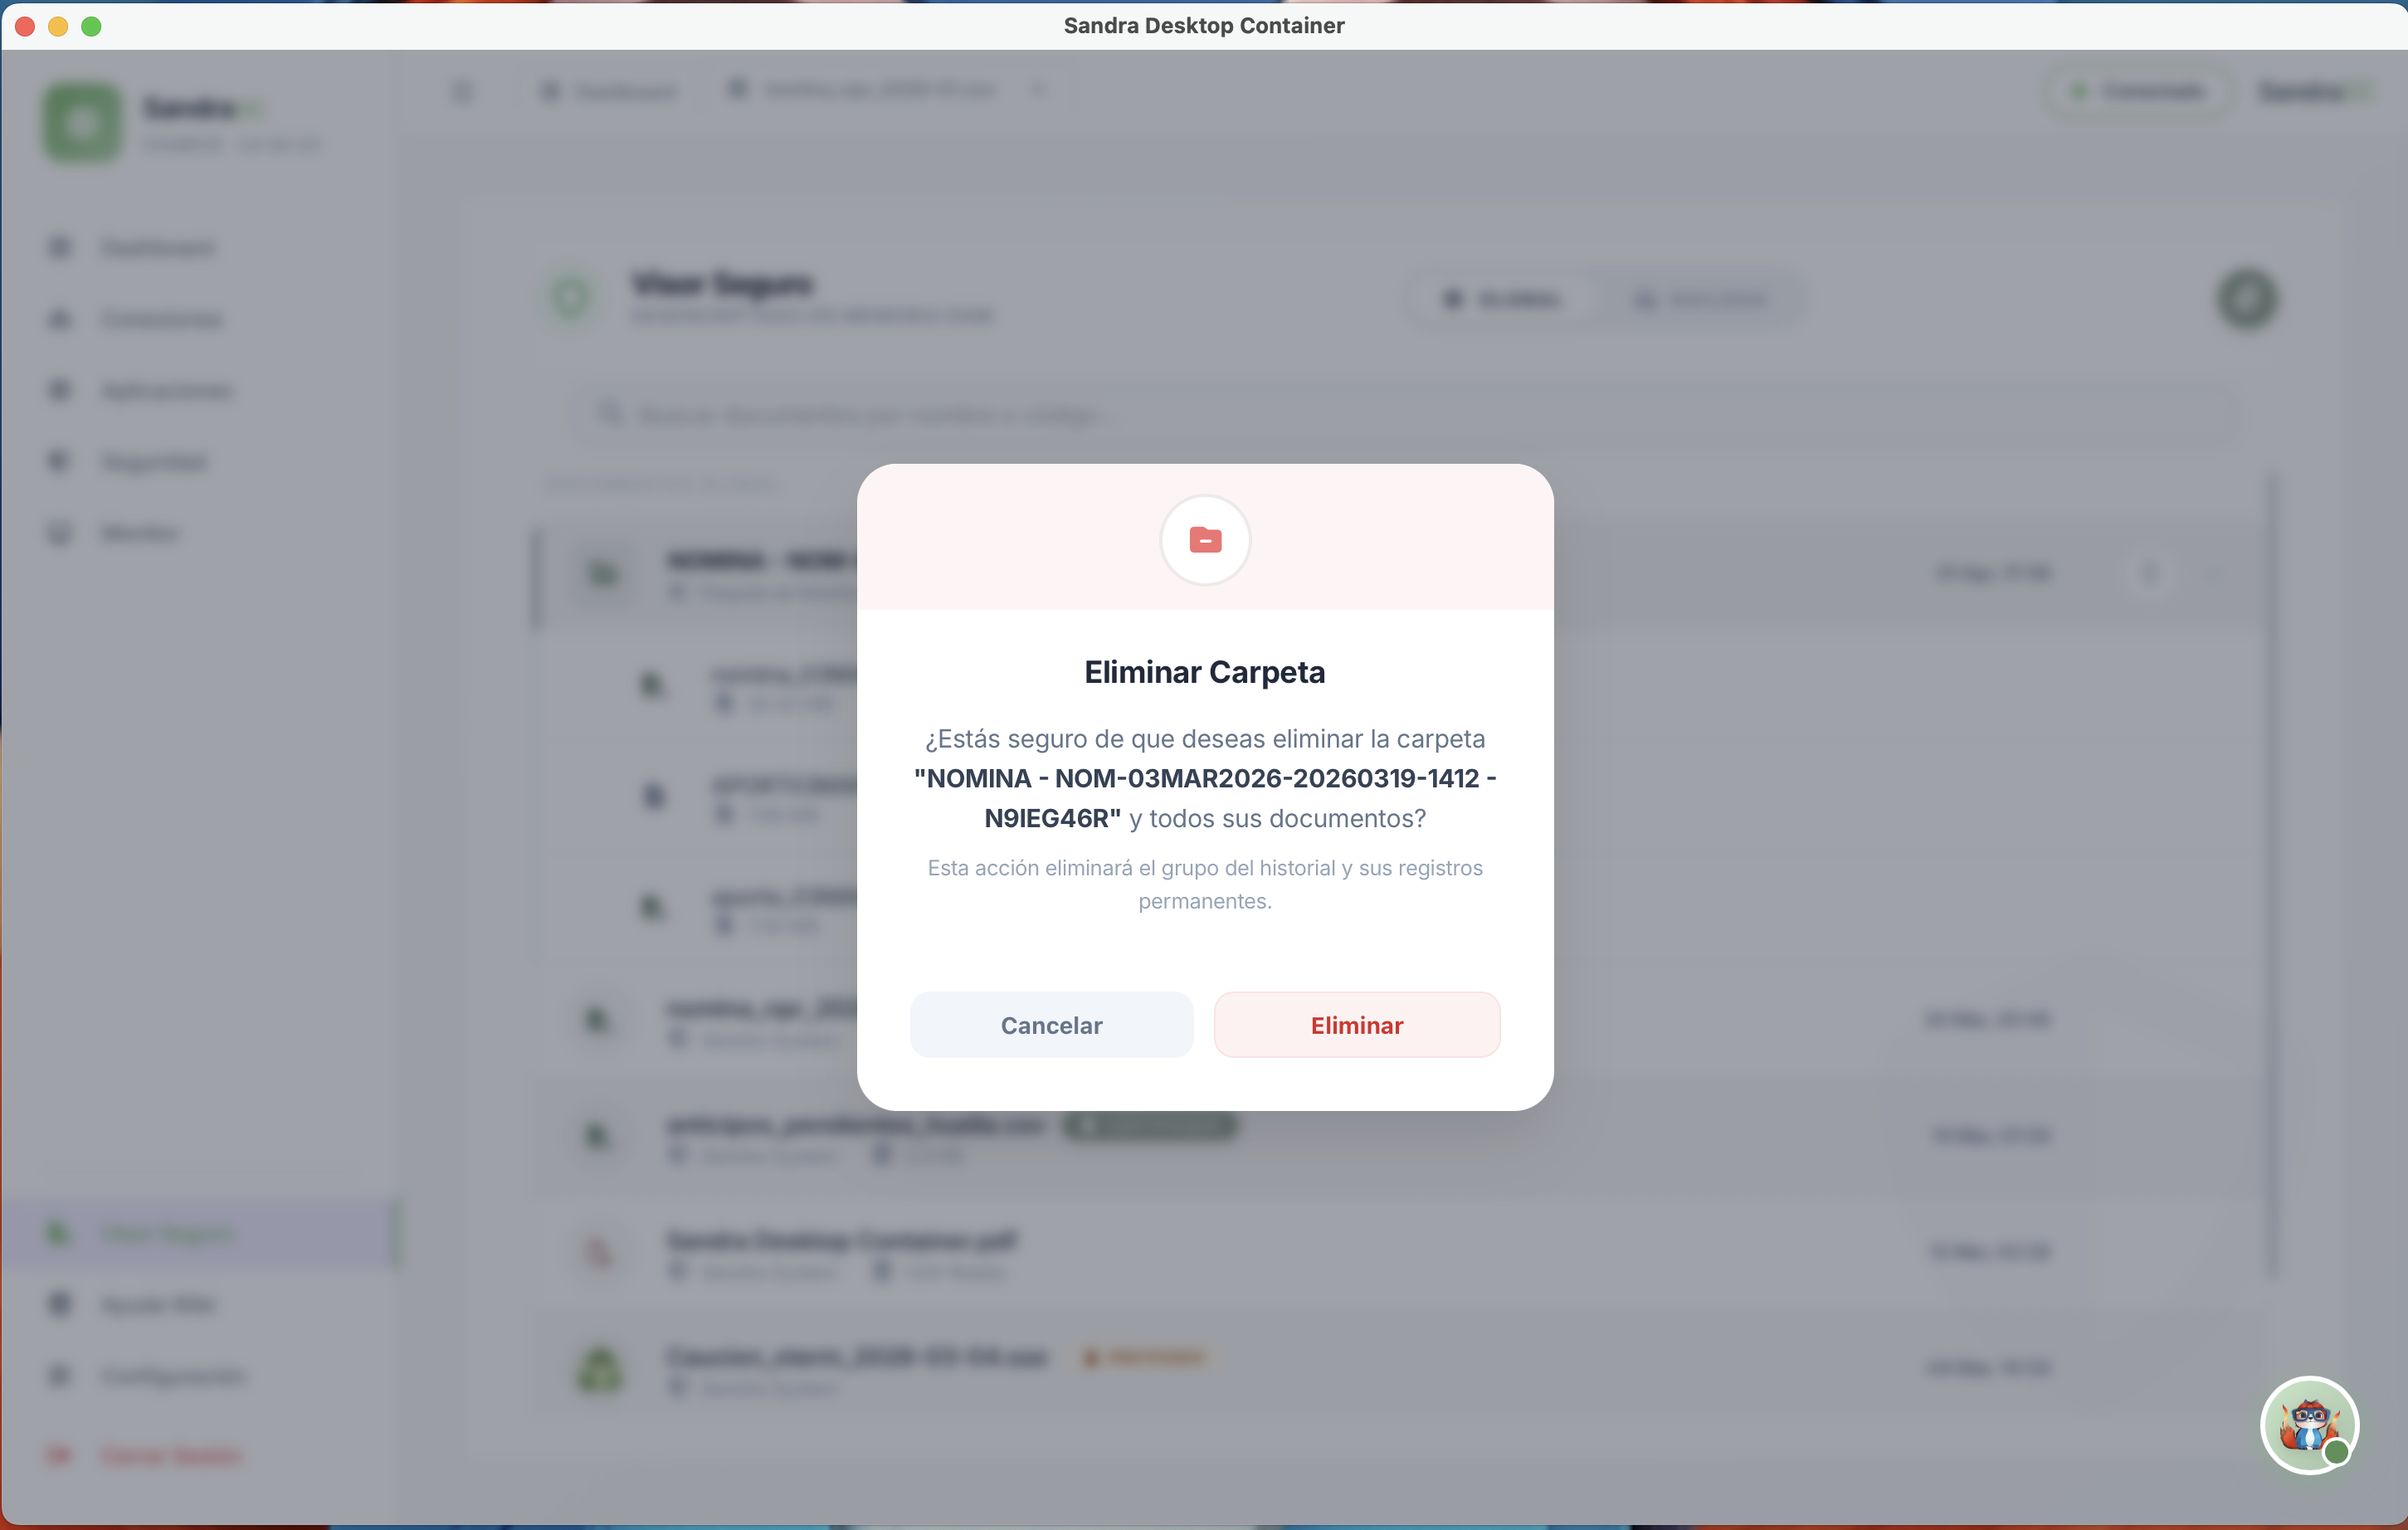
\includegraphics[width=0.7\textwidth]{anexos/11 visor.eliminar.nomina.png}}
\caption{Panel de eliminacion segura de documentos}
\label{fig:visor-eliminar}
\end{figure}

\subsection{Proceso de Eliminacion Segura}

\begin{enumerate}
    \item El usuario selecciona el documento a eliminar
    \item SDC muestra confirmacion con resumen del documento
    \item Se ejecuta borrado seguro (overwrite con datos aleatorios)
    \item Se elimina la referencia de la base de datos
    \item Se registra el evento en logs de auditoria
\end{enumerate}

\begin{caja}{Trazabilidad de Eliminacion}
Cada eliminacion genera un registro de auditoria que incluye:
\begin{itemize}[leftmargin=1.5em, nosep]
    \item Usuario que realizo la eliminacion
    \item Timestamp del evento
    \item Hash del documento eliminado
    \item Motivo de eliminacion (si se especifica)
\end{itemize}
\end{caja}

\notacientifica{Los documentos eliminados no pueden ser recuperados ni por el usuario ni por administradores del sistema.}

\section{Estados del Visor}
\label{sec:estados-visor}

El visor muestra diferentes estados durante su ciclo de vida:

\begin{figure}[H]
\centering
\fbox{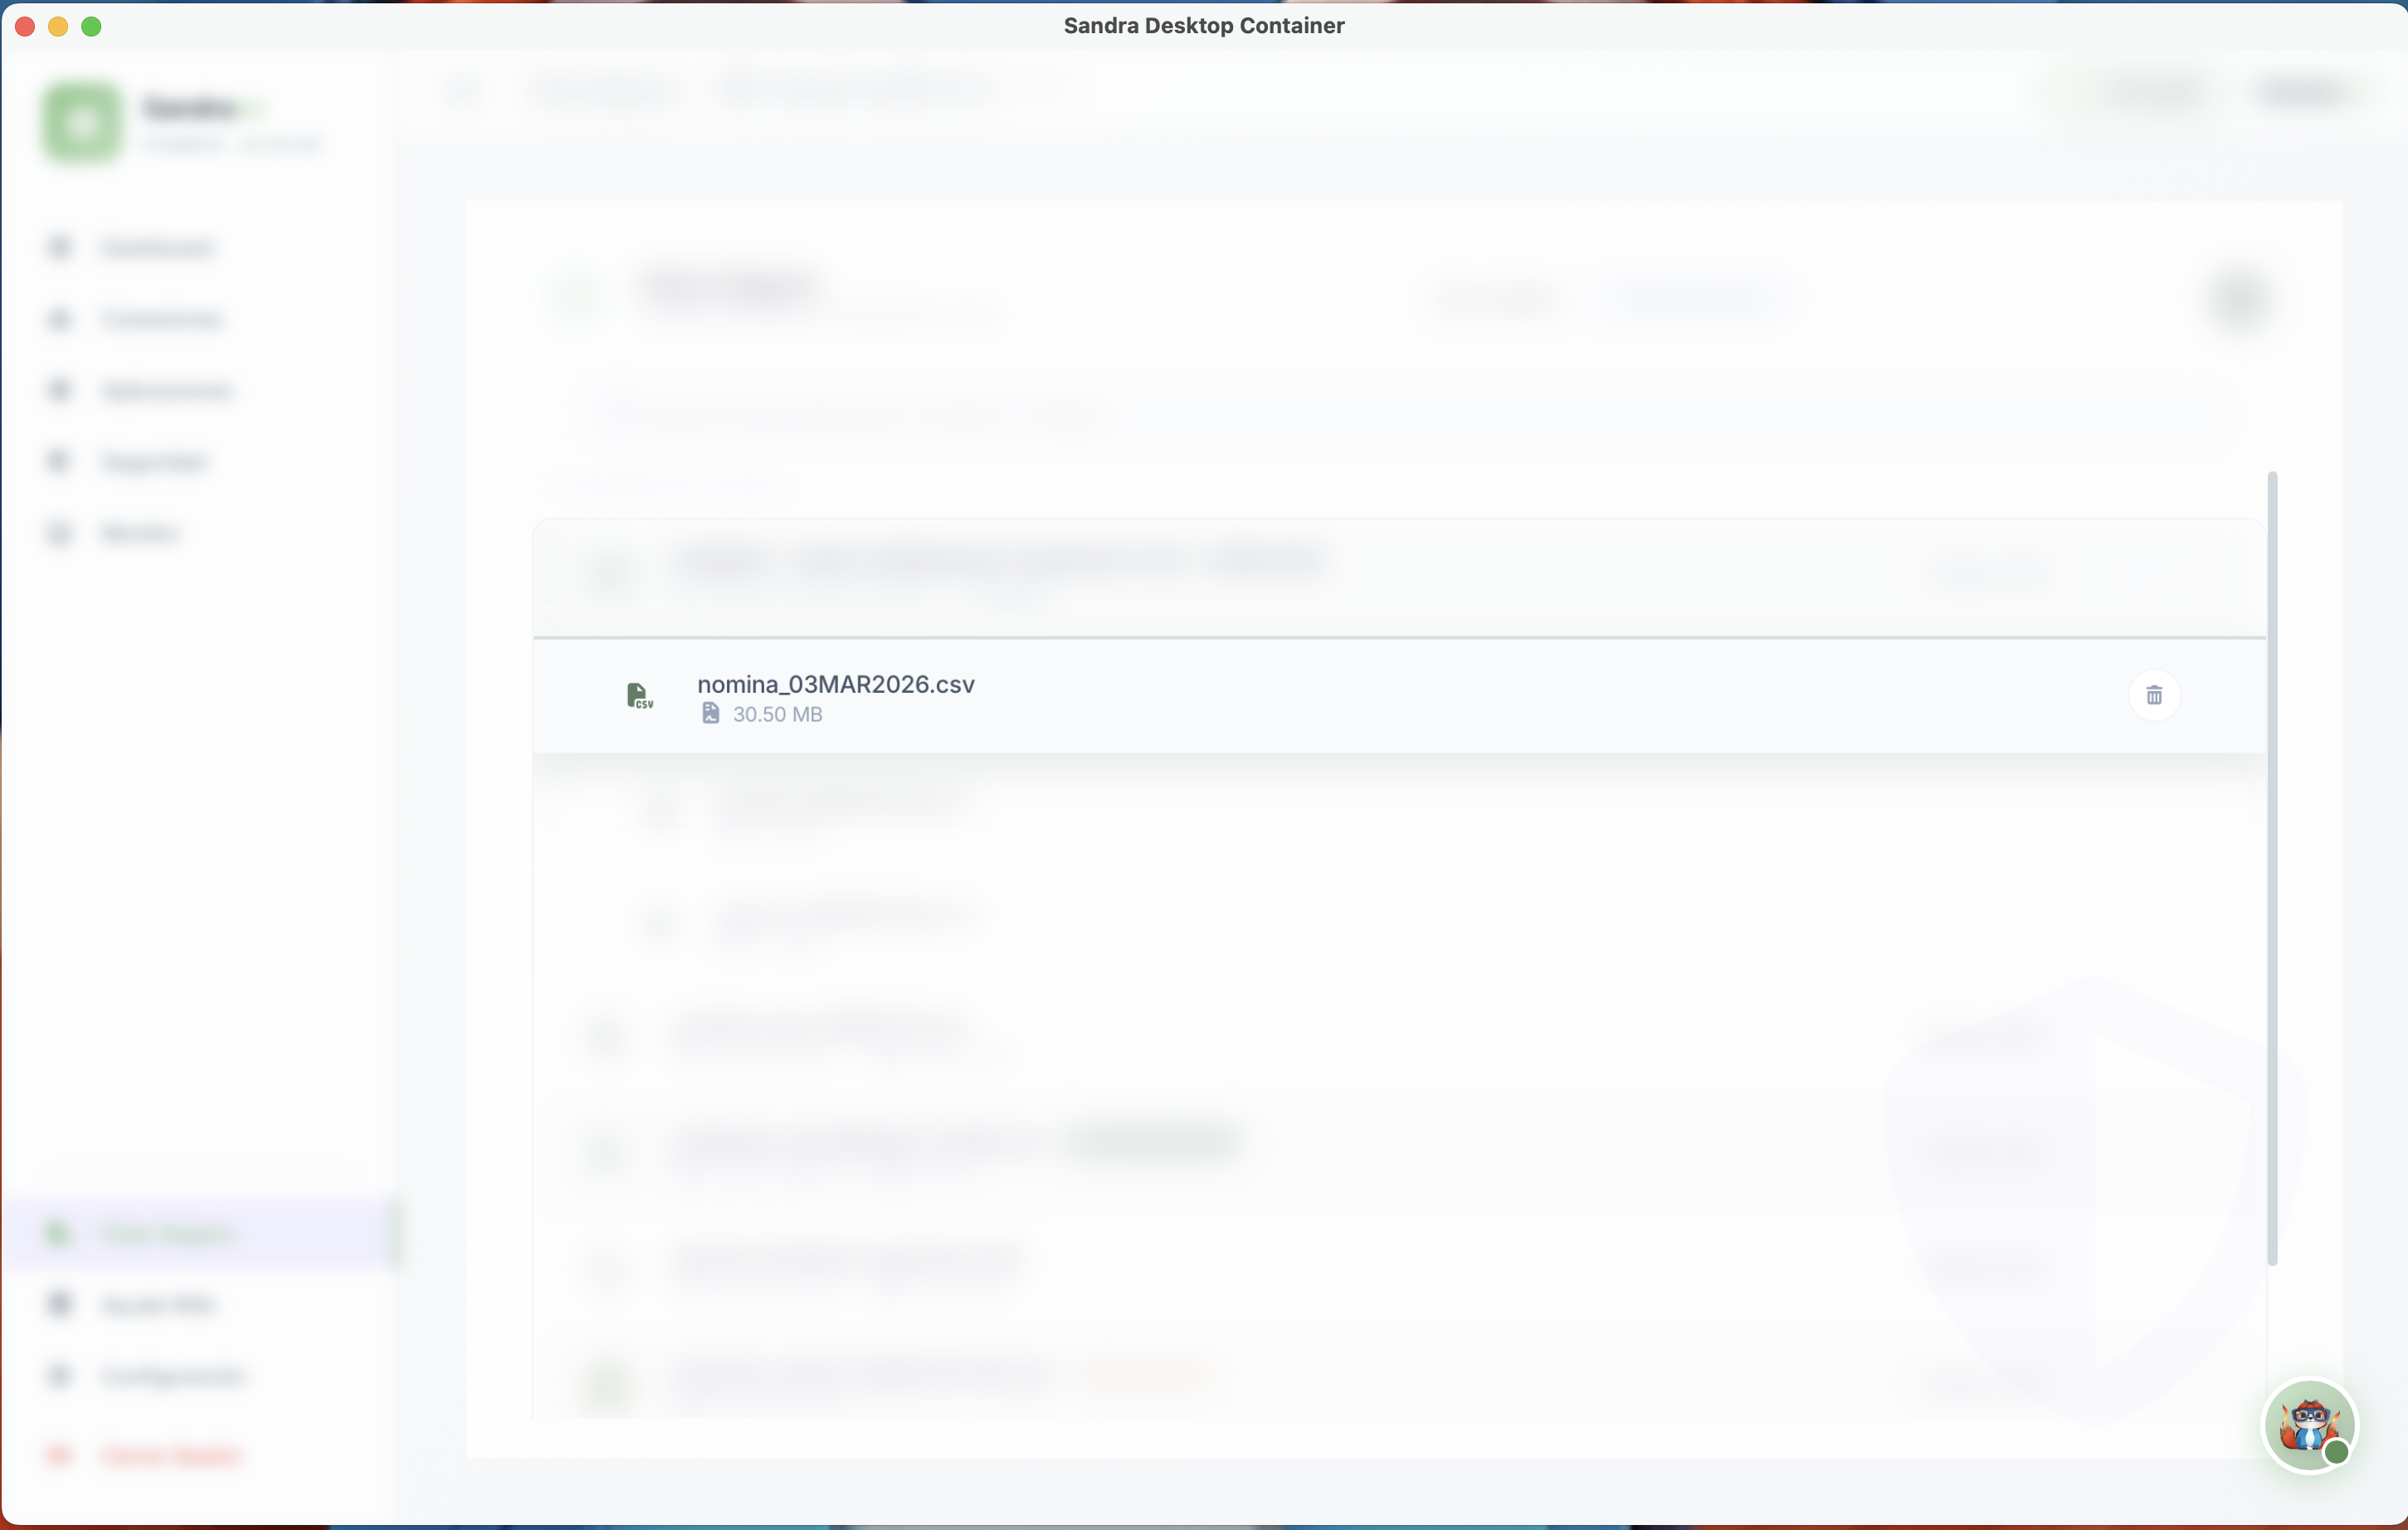
\includegraphics[width=0.65\textwidth]{anexos/11 visor.cargando.png}}
\caption{Estado de carga del documento}
\label{fig:visor-cargando}
\end{figure}

\subsection{Estado: Cargando}

\begin{itemize}[leftmargin=*]
    \item Indicador de progreso de descarga
    \item Descompresion de archivos comprimidos
    \item Verificacion de integridad del documento
    \item Preparacion del buffer de visualizacion
\end{itemize}

\begin{figure}[H]
\centering
\fbox{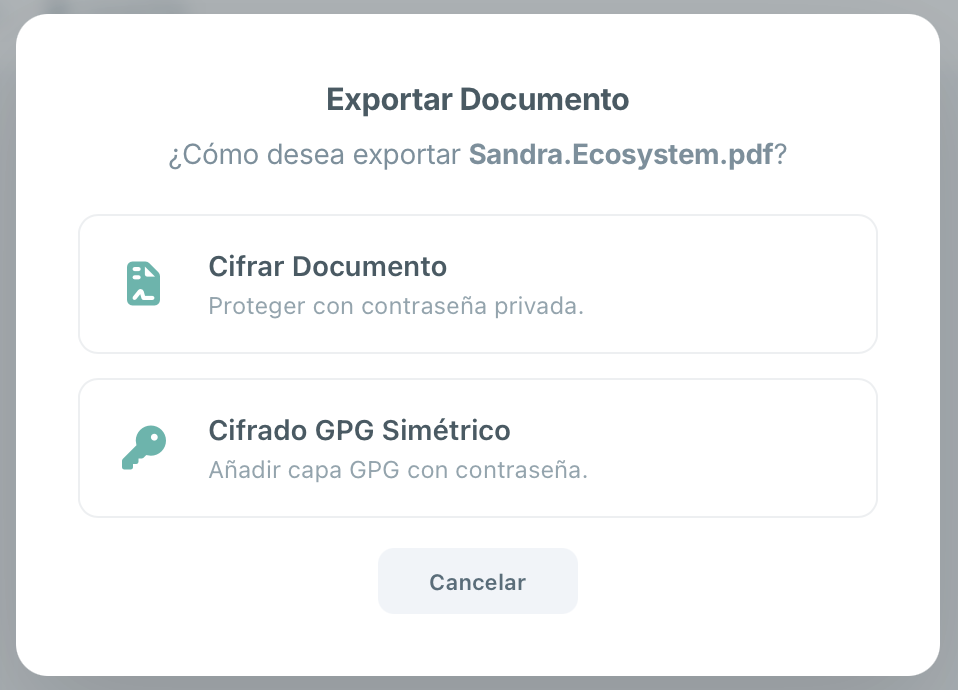
\includegraphics[width=0.65\textwidth]{anexos/14 visor encriptado.png}}
\caption{Estado de documento encriptado}
\label{fig:visor-encriptado-estado}
\end{figure}

\subsection{Estado: Encriptado}

\begin{itemize}[leftmargin=*]
    \item Indicador de candado activo
    \item Requerimiento de clave para acceso
    \item Vista previa de metadatos (sin contenido)
    \item Opciones de desbloqueo disponibles
\end{itemize}

\notacientifica{El cambio entre estados es automatico y no requiere intervencion del usuario.}

\section{Exportacion Avanzada}
\label{sec:export-avanzada}

\subsection{Exportacion GPG}

\begin{figure}[H]
\centering
\fbox{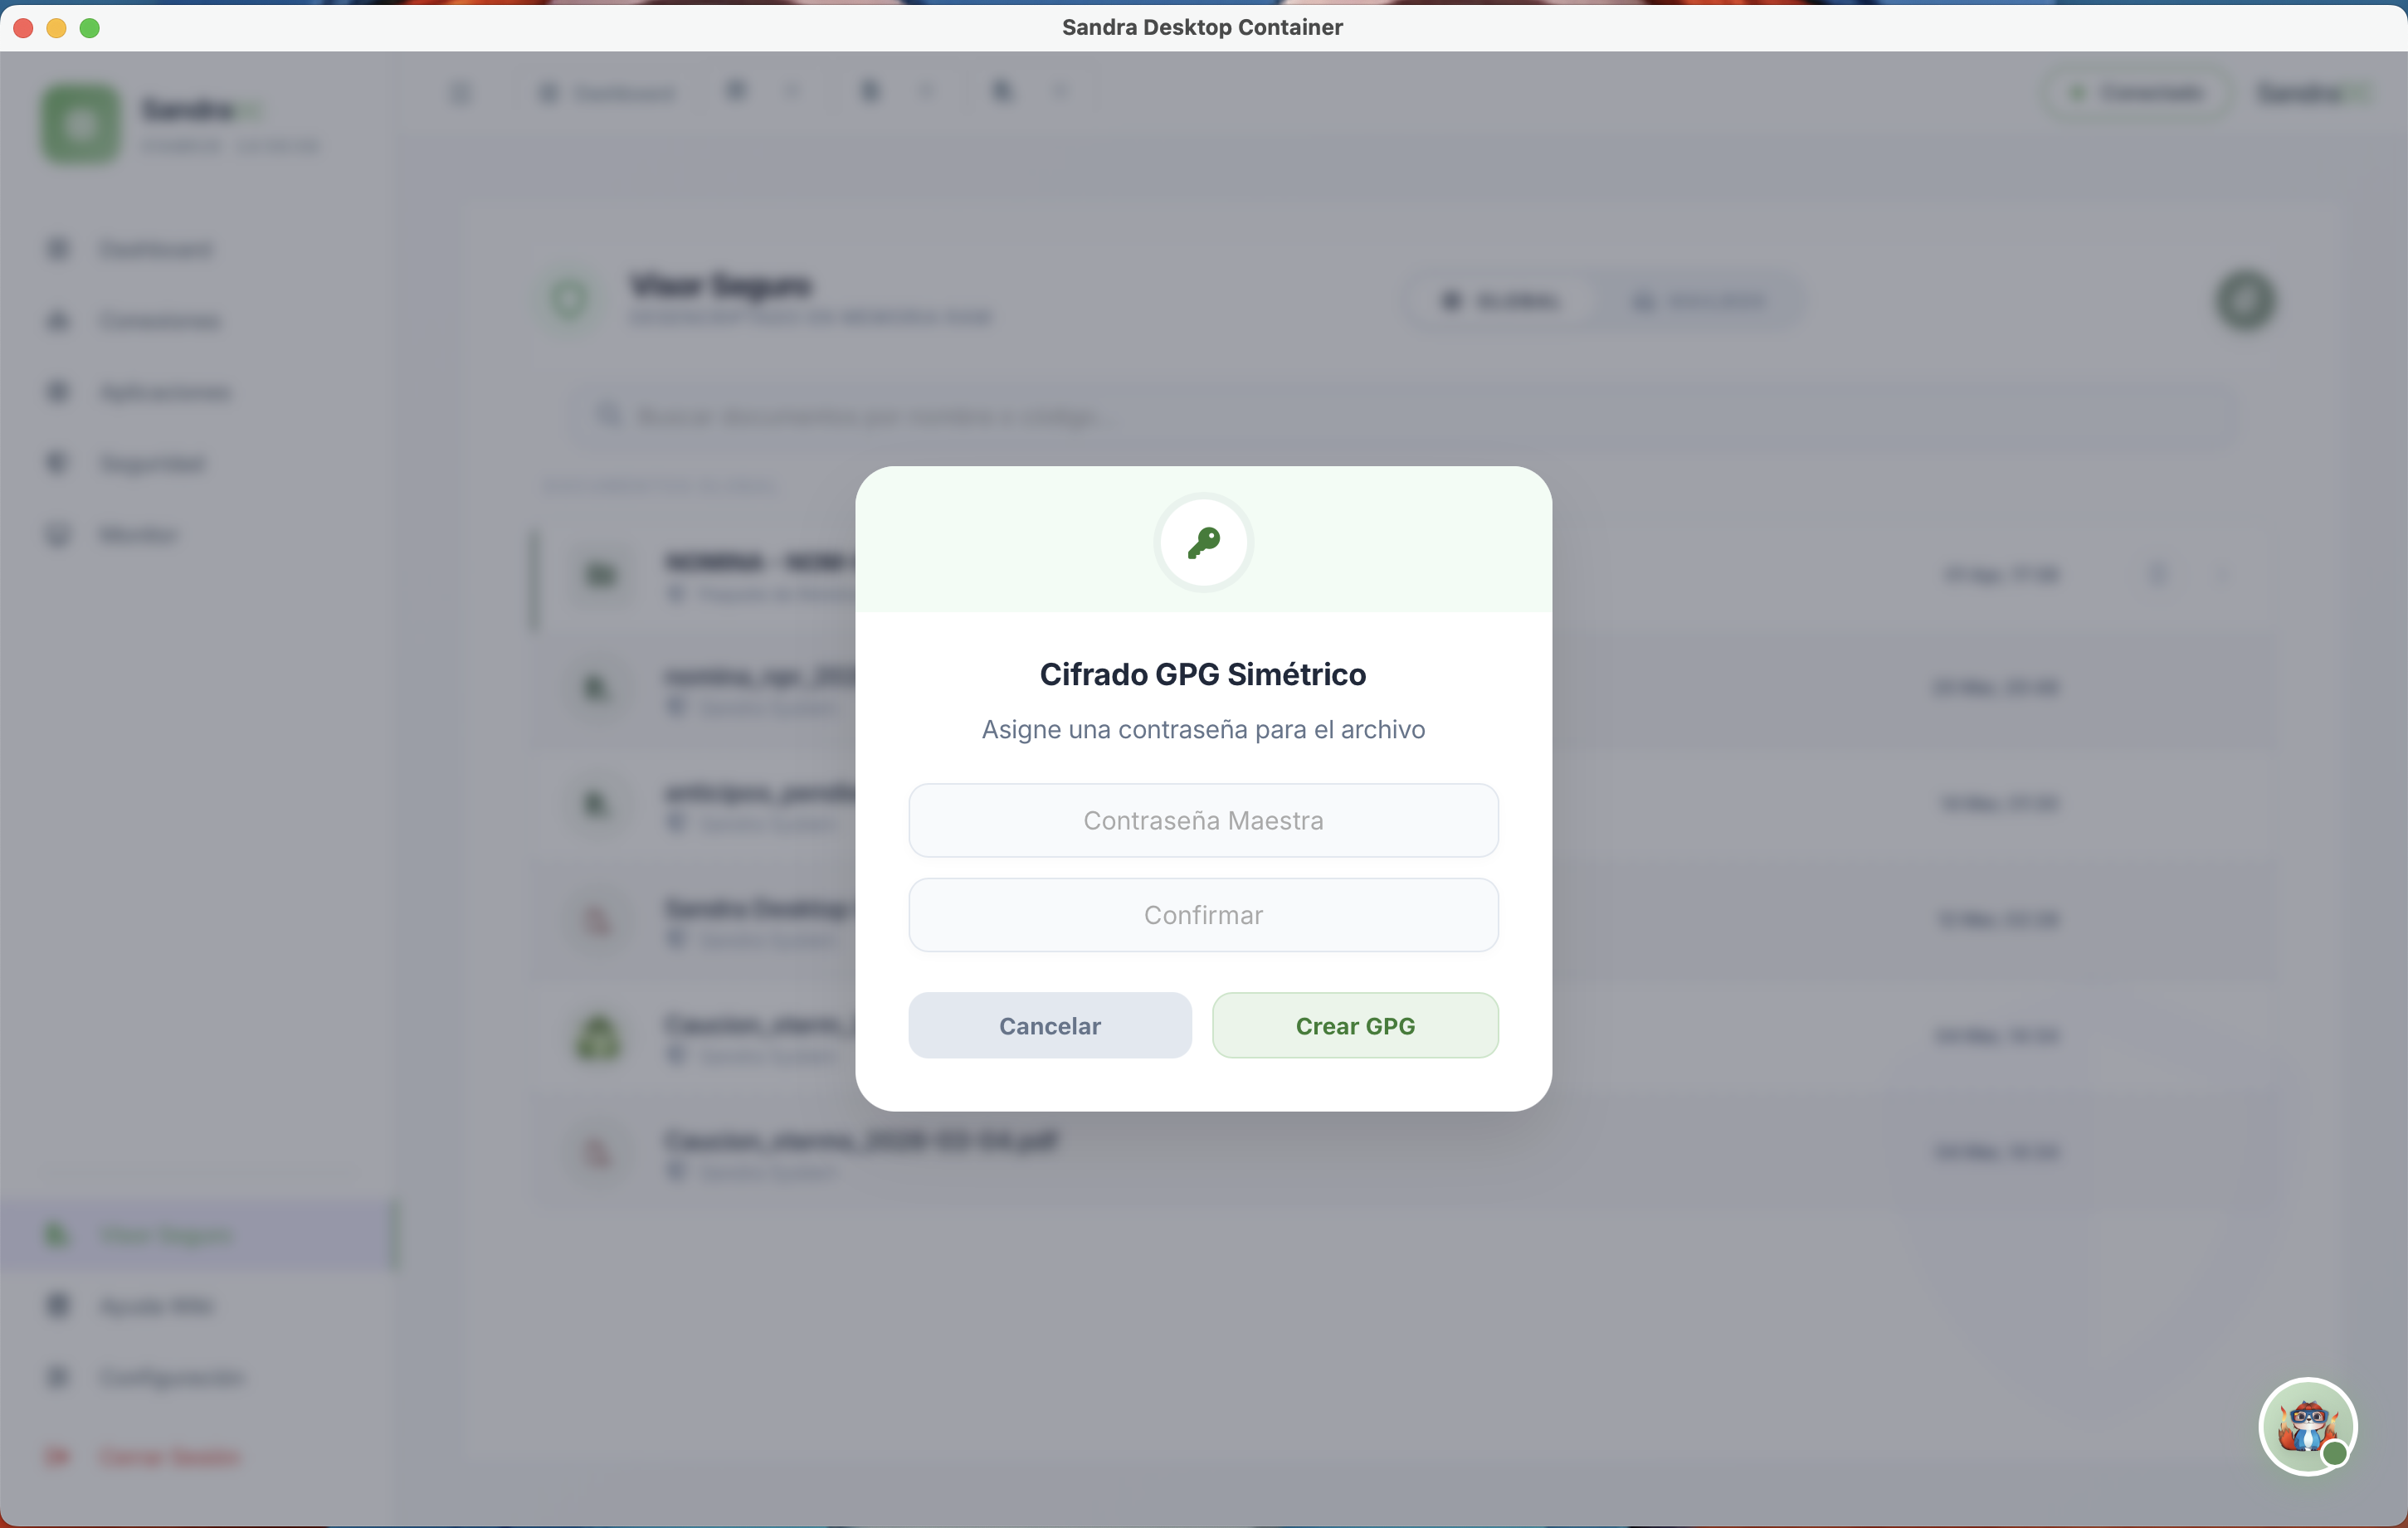
\includegraphics[width=0.65\textwidth]{anexos/11 visor encriptar.gpg.png}}
\caption{Exportacion con formato GPG}
\label{fig:visor-export-gpg}
\end{figure}

El sistema permite exportar documentos con cifrado GPG:

\begin{caja}{Opciones de Exportacion GPG}
\begin{itemize}[leftmargin=1.5em, nosep]
    \item \textbf{Cifrado simetrico}: Con passphrase definida por el usuario
    \item \textbf{Cifrado asimetrico}: Con clave publica del destinatario
    \item \textbf{Firma separada}: Genera archivo .sig adjunto
    \item \textbf{Formato armored}: Salida ASCII readable (para email)
\end{itemize}
\end{caja}

\notacientifica{Los archivos exportados en formato GPG son interoperables con cualquier sistema compatible OpenPGP.}

\subsection{Exportacion SSE (Server-Side Encryption)}

\begin{figure}[H]
\centering
\fbox{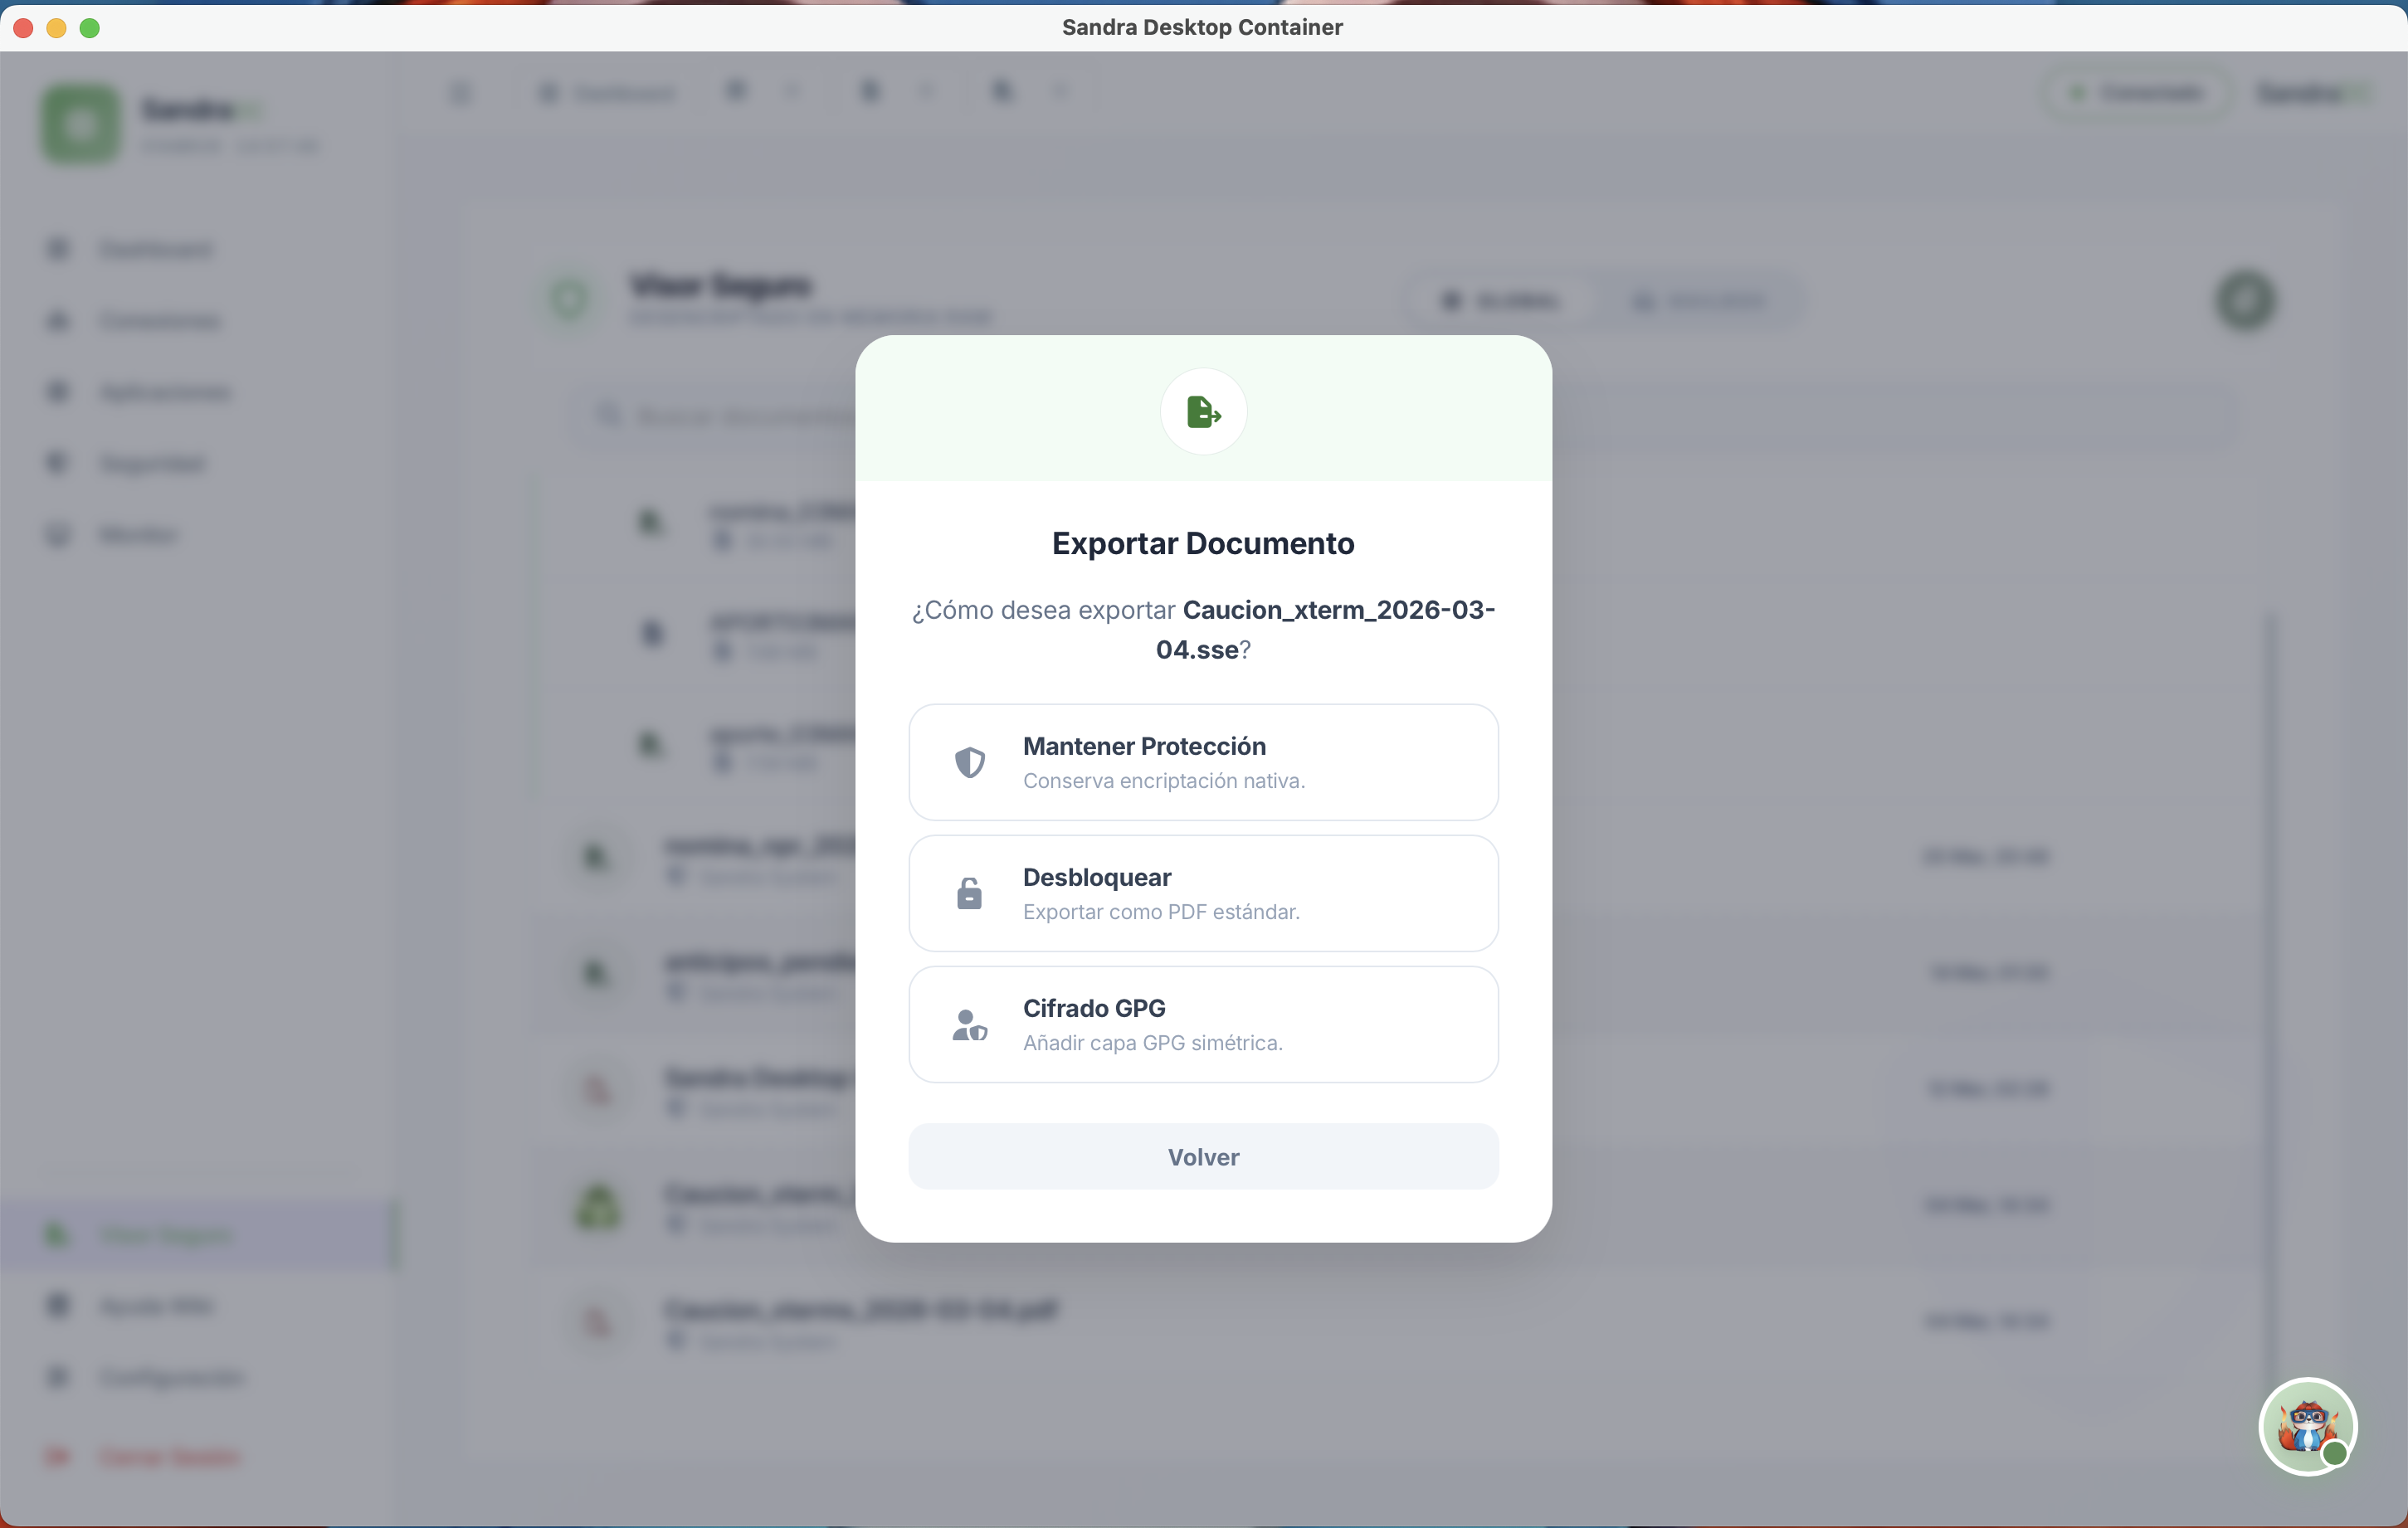
\includegraphics[width=0.65\textwidth]{anexos/11 visor exportar.sse.png}}
\caption{Exportacion con cifrado del lado del servidor}
\label{fig:visor-export-sse}
\end{figure}

La exportacion SSE proporciona:

\begin{itemize}[leftmargin=*]
    \item Cifrado con claves gestionadas por SDC
    \item Posibilidad de agregar sello de trazabilidad
    \item Registro de auditoria de la exportacion
    \item Revocacion de acceso via URL
\end{itemize}

\notacientifica{La combinacion de SSE + Sello de Alquimia Invisible proporciona maxima proteccion para documentos sensibles.}
